\documentclass[12pt]{article}
\usepackage[letterpaper, margin=0.7in, headheight=15pt, headsep=14pt, footskip=26pt, includeheadfoot=false]{geometry}
\usepackage[T1]{fontenc}
\usepackage{tgheros}
\renewcommand{\familydefault}{\sfdefault}
\usepackage{tikz}
\usetikzlibrary{arrows.meta}
\usepackage{fancyhdr}
\pagestyle{fancy}
\fancyhf{}
\fancyhead[L]{Week 66 / Lamplighter streets / K--1}
\fancyfoot[L]{Bellingham Math Circle / Week 66 / GGT66-K-v1}
\fancyfoot[R]{\thepage}
\renewcommand{\headrulewidth}{0pt}
\setlength{\parindent}{0pt}
\linespread{1.12}
\begin{document}
\noindent\begin{minipage}[t]{0.62\textwidth}\vspace{0pt}
Start every try with all lamps off and the walker at home. A move is one step left, one step right, or a flip of the lamp under the walker. One partner moves the walker. The other points to the lamp under the walker, then flips it. Swap jobs for each new picture. Put one cube on your tower for each move. Color one square under the picture for each cube in your shortest tower.
\end{minipage}\hfill\begin{minipage}[t]{0.345\textwidth}\vspace{1mm}\centering
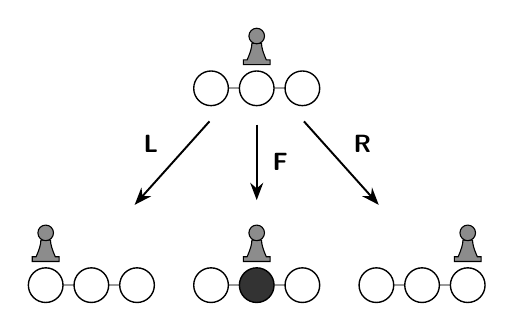
\begin{tikzpicture}[x=1mm, y=1mm]
\draw[line width=0.7pt, black!40] (-5.80,0.00) -- (5.80,0.00);
\draw[line width=0.5pt, fill=white] (-5.80,0.00) circle (2.2);
\draw[line width=0.5pt, fill=white] (0.00,0.00) circle (2.2);
\draw[line width=0.5pt, fill=white] (5.80,0.00) circle (2.2);
\draw[line width=0.4pt, fill=black!45] (-1.70,3.00) -- (1.70,3.00) -- (1.70,3.61) -- (1.22,3.61) .. controls (0.82,4.50) and (0.61,5.18) .. (0.61,5.72) -- (-0.61,5.72) .. controls (-0.61,5.18) and (-0.82,4.50) .. (-1.22,3.61) -- (-1.70,3.61) -- cycle;
\draw[line width=0.4pt, fill=black!45] (0.00,6.64) circle (0.99);
\draw[line width=0.7pt, black!40] (-26.80,-25.00) -- (-15.20,-25.00);
\draw[line width=0.5pt, fill=white] (-26.80,-25.00) circle (2.2);
\draw[line width=0.5pt, fill=white] (-21.00,-25.00) circle (2.2);
\draw[line width=0.5pt, fill=white] (-15.20,-25.00) circle (2.2);
\draw[line width=0.4pt, fill=black!45] (-28.50,-22.00) -- (-25.10,-22.00) -- (-25.10,-21.39) -- (-25.58,-21.39) .. controls (-25.98,-20.50) and (-26.19,-19.82) .. (-26.19,-19.28) -- (-27.41,-19.28) .. controls (-27.41,-19.82) and (-27.62,-20.50) .. (-28.02,-21.39) -- (-28.50,-21.39) -- cycle;
\draw[line width=0.4pt, fill=black!45] (-26.80,-18.36) circle (0.99);
\draw[line width=0.7pt, black!40] (-5.80,-25.00) -- (5.80,-25.00);
\draw[line width=0.5pt, fill=white] (-5.80,-25.00) circle (2.2);
\draw[line width=0.5pt, fill=black!80] (0.00,-25.00) circle (2.2);
\draw[line width=0.5pt, fill=white] (5.80,-25.00) circle (2.2);
\draw[line width=0.4pt, fill=black!45] (-1.70,-22.00) -- (1.70,-22.00) -- (1.70,-21.39) -- (1.22,-21.39) .. controls (0.82,-20.50) and (0.61,-19.82) .. (0.61,-19.28) -- (-0.61,-19.28) .. controls (-0.61,-19.82) and (-0.82,-20.50) .. (-1.22,-21.39) -- (-1.70,-21.39) -- cycle;
\draw[line width=0.4pt, fill=black!45] (0.00,-18.36) circle (0.99);
\draw[line width=0.7pt, black!40] (15.20,-25.00) -- (26.80,-25.00);
\draw[line width=0.5pt, fill=white] (15.20,-25.00) circle (2.2);
\draw[line width=0.5pt, fill=white] (21.00,-25.00) circle (2.2);
\draw[line width=0.5pt, fill=white] (26.80,-25.00) circle (2.2);
\draw[line width=0.4pt, fill=black!45] (25.10,-22.00) -- (28.50,-22.00) -- (28.50,-21.39) -- (28.02,-21.39) .. controls (27.62,-20.50) and (27.41,-19.82) .. (27.41,-19.28) -- (26.19,-19.28) .. controls (26.19,-19.82) and (25.98,-20.50) .. (25.58,-21.39) -- (25.10,-21.39) -- cycle;
\draw[line width=0.4pt, fill=black!45] (26.80,-18.36) circle (0.99);
\draw[-{Stealth[length=2.2mm]}, line width=0.7pt] (-6.00,-4.20) -- (-15.50,-14.80);
\node[font=\sffamily\bfseries\small, inner sep=0pt] at (-13.43,-7.10) {L};
\draw[-{Stealth[length=2.2mm]}, line width=0.7pt] (6.00,-4.20) -- (15.50,-14.80);
\node[font=\sffamily\bfseries\small, inner sep=0pt] at (13.43,-7.10) {R};
\draw[-{Stealth[length=2.2mm]}, line width=0.7pt] (0.00,-4.60) -- (0.00,-14.20);
\node[font=\sffamily\bfseries\small, inner sep=0pt] at (3.00,-9.40) {F};
\end{tikzpicture}
\end{minipage}

\vspace{6mm}\noindent\textbf{Problem 1:} Build each picture with as few moves as you can.

\vspace{5mm}\centerline{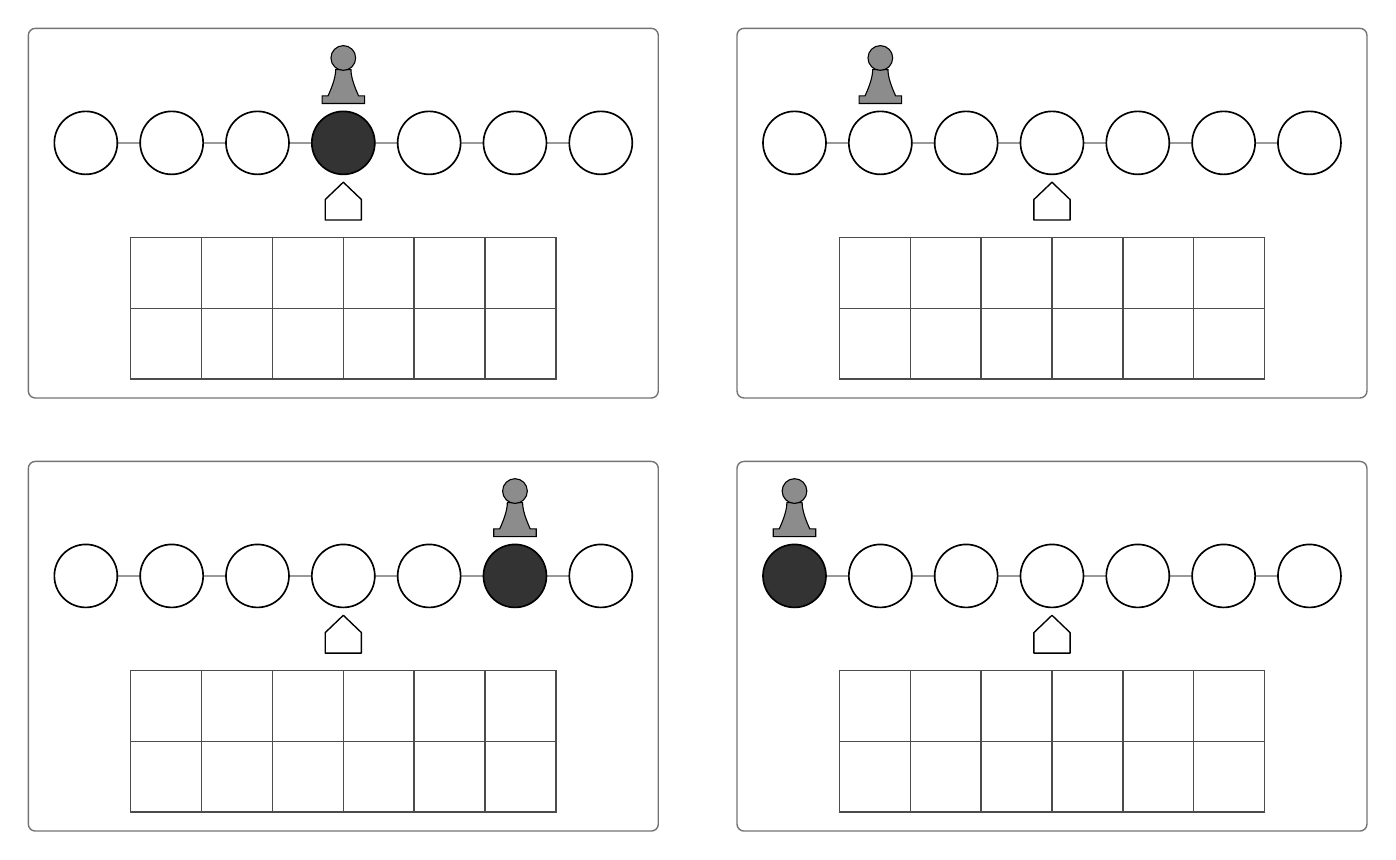
\begin{tikzpicture}[x=1mm, y=1mm]
\draw[line width=0.5pt, black!55, rounded corners=2.5] (-85.00,-32.40) rectangle (-5.00,14.54);
\draw[line width=0.9pt, black!40] (-77.70,0.00) -- (-12.30,0.00);
\draw[line width=0.6pt, fill=white] (-77.70,0.00) circle (4.0);
\draw[line width=0.6pt, fill=white] (-66.80,0.00) circle (4.0);
\draw[line width=0.6pt, fill=white] (-55.90,0.00) circle (4.0);
\draw[line width=0.6pt, fill=black!80] (-45.00,0.00) circle (4.0);
\draw[line width=0.6pt, fill=white] (-34.10,0.00) circle (4.0);
\draw[line width=0.6pt, fill=white] (-23.20,0.00) circle (4.0);
\draw[line width=0.6pt, fill=white] (-12.30,0.00) circle (4.0);
\draw[line width=0.4pt, fill=black!45] (-47.70,5.00) -- (-42.30,5.00) -- (-42.30,5.97) -- (-43.06,5.97) .. controls (-43.70,7.38) and (-44.03,8.46) .. (-44.03,9.32) -- (-45.97,9.32) .. controls (-45.97,8.46) and (-46.30,7.38) .. (-46.94,5.97) -- (-47.70,5.97) -- cycle;
\draw[line width=0.4pt, fill=black!45] (-45.00,10.78) circle (1.57);
\draw[line width=0.5pt, line join=round] (-45.00,-5.00) -- (-42.70,-7.20) -- (-42.70,-9.80) -- (-47.30,-9.80) -- (-47.30,-7.20) -- cycle;
\draw[line width=0.5pt, black!70] (-72.00,-21.00) rectangle (-63.00,-12.00);
\draw[line width=0.5pt, black!70] (-63.00,-21.00) rectangle (-54.00,-12.00);
\draw[line width=0.5pt, black!70] (-54.00,-21.00) rectangle (-45.00,-12.00);
\draw[line width=0.5pt, black!70] (-45.00,-21.00) rectangle (-36.00,-12.00);
\draw[line width=0.5pt, black!70] (-36.00,-21.00) rectangle (-27.00,-12.00);
\draw[line width=0.5pt, black!70] (-27.00,-21.00) rectangle (-18.00,-12.00);
\draw[line width=0.5pt, black!70] (-72.00,-30.00) rectangle (-63.00,-21.00);
\draw[line width=0.5pt, black!70] (-63.00,-30.00) rectangle (-54.00,-21.00);
\draw[line width=0.5pt, black!70] (-54.00,-30.00) rectangle (-45.00,-21.00);
\draw[line width=0.5pt, black!70] (-45.00,-30.00) rectangle (-36.00,-21.00);
\draw[line width=0.5pt, black!70] (-36.00,-30.00) rectangle (-27.00,-21.00);
\draw[line width=0.5pt, black!70] (-27.00,-30.00) rectangle (-18.00,-21.00);
\draw[line width=0.5pt, black!55, rounded corners=2.5] (5.00,-32.40) rectangle (85.00,14.54);
\draw[line width=0.9pt, black!40] (12.30,0.00) -- (77.70,0.00);
\draw[line width=0.6pt, fill=white] (12.30,0.00) circle (4.0);
\draw[line width=0.6pt, fill=white] (23.20,0.00) circle (4.0);
\draw[line width=0.6pt, fill=white] (34.10,0.00) circle (4.0);
\draw[line width=0.6pt, fill=white] (45.00,0.00) circle (4.0);
\draw[line width=0.6pt, fill=white] (55.90,0.00) circle (4.0);
\draw[line width=0.6pt, fill=white] (66.80,0.00) circle (4.0);
\draw[line width=0.6pt, fill=white] (77.70,0.00) circle (4.0);
\draw[line width=0.4pt, fill=black!45] (20.50,5.00) -- (25.90,5.00) -- (25.90,5.97) -- (25.14,5.97) .. controls (24.50,7.38) and (24.17,8.46) .. (24.17,9.32) -- (22.23,9.32) .. controls (22.23,8.46) and (21.90,7.38) .. (21.26,5.97) -- (20.50,5.97) -- cycle;
\draw[line width=0.4pt, fill=black!45] (23.20,10.78) circle (1.57);
\draw[line width=0.5pt, line join=round] (45.00,-5.00) -- (47.30,-7.20) -- (47.30,-9.80) -- (42.70,-9.80) -- (42.70,-7.20) -- cycle;
\draw[line width=0.5pt, black!70] (18.00,-21.00) rectangle (27.00,-12.00);
\draw[line width=0.5pt, black!70] (27.00,-21.00) rectangle (36.00,-12.00);
\draw[line width=0.5pt, black!70] (36.00,-21.00) rectangle (45.00,-12.00);
\draw[line width=0.5pt, black!70] (45.00,-21.00) rectangle (54.00,-12.00);
\draw[line width=0.5pt, black!70] (54.00,-21.00) rectangle (63.00,-12.00);
\draw[line width=0.5pt, black!70] (63.00,-21.00) rectangle (72.00,-12.00);
\draw[line width=0.5pt, black!70] (18.00,-30.00) rectangle (27.00,-21.00);
\draw[line width=0.5pt, black!70] (27.00,-30.00) rectangle (36.00,-21.00);
\draw[line width=0.5pt, black!70] (36.00,-30.00) rectangle (45.00,-21.00);
\draw[line width=0.5pt, black!70] (45.00,-30.00) rectangle (54.00,-21.00);
\draw[line width=0.5pt, black!70] (54.00,-30.00) rectangle (63.00,-21.00);
\draw[line width=0.5pt, black!70] (63.00,-30.00) rectangle (72.00,-21.00);
\draw[line width=0.5pt, black!55, rounded corners=2.5] (-85.00,-87.40) rectangle (-5.00,-40.46);
\draw[line width=0.9pt, black!40] (-77.70,-55.00) -- (-12.30,-55.00);
\draw[line width=0.6pt, fill=white] (-77.70,-55.00) circle (4.0);
\draw[line width=0.6pt, fill=white] (-66.80,-55.00) circle (4.0);
\draw[line width=0.6pt, fill=white] (-55.90,-55.00) circle (4.0);
\draw[line width=0.6pt, fill=white] (-45.00,-55.00) circle (4.0);
\draw[line width=0.6pt, fill=white] (-34.10,-55.00) circle (4.0);
\draw[line width=0.6pt, fill=black!80] (-23.20,-55.00) circle (4.0);
\draw[line width=0.6pt, fill=white] (-12.30,-55.00) circle (4.0);
\draw[line width=0.4pt, fill=black!45] (-25.90,-50.00) -- (-20.50,-50.00) -- (-20.50,-49.03) -- (-21.26,-49.03) .. controls (-21.90,-47.62) and (-22.23,-46.54) .. (-22.23,-45.68) -- (-24.17,-45.68) .. controls (-24.17,-46.54) and (-24.50,-47.62) .. (-25.14,-49.03) -- (-25.90,-49.03) -- cycle;
\draw[line width=0.4pt, fill=black!45] (-23.20,-44.22) circle (1.57);
\draw[line width=0.5pt, line join=round] (-45.00,-60.00) -- (-42.70,-62.20) -- (-42.70,-64.80) -- (-47.30,-64.80) -- (-47.30,-62.20) -- cycle;
\draw[line width=0.5pt, black!70] (-72.00,-76.00) rectangle (-63.00,-67.00);
\draw[line width=0.5pt, black!70] (-63.00,-76.00) rectangle (-54.00,-67.00);
\draw[line width=0.5pt, black!70] (-54.00,-76.00) rectangle (-45.00,-67.00);
\draw[line width=0.5pt, black!70] (-45.00,-76.00) rectangle (-36.00,-67.00);
\draw[line width=0.5pt, black!70] (-36.00,-76.00) rectangle (-27.00,-67.00);
\draw[line width=0.5pt, black!70] (-27.00,-76.00) rectangle (-18.00,-67.00);
\draw[line width=0.5pt, black!70] (-72.00,-85.00) rectangle (-63.00,-76.00);
\draw[line width=0.5pt, black!70] (-63.00,-85.00) rectangle (-54.00,-76.00);
\draw[line width=0.5pt, black!70] (-54.00,-85.00) rectangle (-45.00,-76.00);
\draw[line width=0.5pt, black!70] (-45.00,-85.00) rectangle (-36.00,-76.00);
\draw[line width=0.5pt, black!70] (-36.00,-85.00) rectangle (-27.00,-76.00);
\draw[line width=0.5pt, black!70] (-27.00,-85.00) rectangle (-18.00,-76.00);
\draw[line width=0.5pt, black!55, rounded corners=2.5] (5.00,-87.40) rectangle (85.00,-40.46);
\draw[line width=0.9pt, black!40] (12.30,-55.00) -- (77.70,-55.00);
\draw[line width=0.6pt, fill=black!80] (12.30,-55.00) circle (4.0);
\draw[line width=0.6pt, fill=white] (23.20,-55.00) circle (4.0);
\draw[line width=0.6pt, fill=white] (34.10,-55.00) circle (4.0);
\draw[line width=0.6pt, fill=white] (45.00,-55.00) circle (4.0);
\draw[line width=0.6pt, fill=white] (55.90,-55.00) circle (4.0);
\draw[line width=0.6pt, fill=white] (66.80,-55.00) circle (4.0);
\draw[line width=0.6pt, fill=white] (77.70,-55.00) circle (4.0);
\draw[line width=0.4pt, fill=black!45] (9.60,-50.00) -- (15.00,-50.00) -- (15.00,-49.03) -- (14.24,-49.03) .. controls (13.60,-47.62) and (13.27,-46.54) .. (13.27,-45.68) -- (11.33,-45.68) .. controls (11.33,-46.54) and (11.00,-47.62) .. (10.36,-49.03) -- (9.60,-49.03) -- cycle;
\draw[line width=0.4pt, fill=black!45] (12.30,-44.22) circle (1.57);
\draw[line width=0.5pt, line join=round] (45.00,-60.00) -- (47.30,-62.20) -- (47.30,-64.80) -- (42.70,-64.80) -- (42.70,-62.20) -- cycle;
\draw[line width=0.5pt, black!70] (18.00,-76.00) rectangle (27.00,-67.00);
\draw[line width=0.5pt, black!70] (27.00,-76.00) rectangle (36.00,-67.00);
\draw[line width=0.5pt, black!70] (36.00,-76.00) rectangle (45.00,-67.00);
\draw[line width=0.5pt, black!70] (45.00,-76.00) rectangle (54.00,-67.00);
\draw[line width=0.5pt, black!70] (54.00,-76.00) rectangle (63.00,-67.00);
\draw[line width=0.5pt, black!70] (63.00,-76.00) rectangle (72.00,-67.00);
\draw[line width=0.5pt, black!70] (18.00,-85.00) rectangle (27.00,-76.00);
\draw[line width=0.5pt, black!70] (27.00,-85.00) rectangle (36.00,-76.00);
\draw[line width=0.5pt, black!70] (36.00,-85.00) rectangle (45.00,-76.00);
\draw[line width=0.5pt, black!70] (45.00,-85.00) rectangle (54.00,-76.00);
\draw[line width=0.5pt, black!70] (54.00,-85.00) rectangle (63.00,-76.00);
\draw[line width=0.5pt, black!70] (63.00,-85.00) rectangle (72.00,-76.00);
\end{tikzpicture}}

\vfill
\centerline{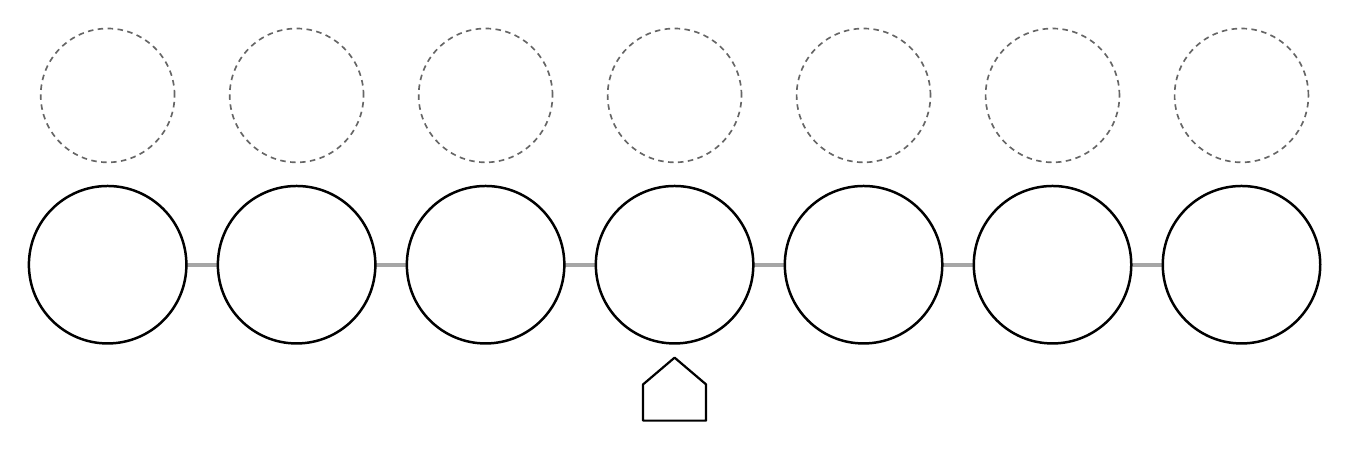
\begin{tikzpicture}[x=1mm, y=1mm]
\draw[line width=1.4pt, black!35] (-78.0,0) -- (78.0,0);
\draw[line width=0.9pt, fill=white] (-72.0,0) circle (10.0);
\draw[line width=0.6pt, black!60, dash pattern=on 2pt off 1.6pt] (-72.0,21.5) circle (8.5);
\draw[line width=0.9pt, fill=white] (-48.0,0) circle (10.0);
\draw[line width=0.6pt, black!60, dash pattern=on 2pt off 1.6pt] (-48.0,21.5) circle (8.5);
\draw[line width=0.9pt, fill=white] (-24.0,0) circle (10.0);
\draw[line width=0.6pt, black!60, dash pattern=on 2pt off 1.6pt] (-24.0,21.5) circle (8.5);
\draw[line width=0.9pt, fill=white] (0.0,0) circle (10.0);
\draw[line width=0.6pt, black!60, dash pattern=on 2pt off 1.6pt] (0.0,21.5) circle (8.5);
\draw[line width=0.9pt, fill=white] (24.0,0) circle (10.0);
\draw[line width=0.6pt, black!60, dash pattern=on 2pt off 1.6pt] (24.0,21.5) circle (8.5);
\draw[line width=0.9pt, fill=white] (48.0,0) circle (10.0);
\draw[line width=0.6pt, black!60, dash pattern=on 2pt off 1.6pt] (48.0,21.5) circle (8.5);
\draw[line width=0.9pt, fill=white] (72.0,0) circle (10.0);
\draw[line width=0.6pt, black!60, dash pattern=on 2pt off 1.6pt] (72.0,21.5) circle (8.5);
\draw[line width=0.8pt, line join=round] (0.00,-11.80) -- (4.00,-15.20) -- (4.00,-19.80) -- (-4.00,-19.80) -- (-4.00,-15.20) -- cycle;
\end{tikzpicture}}
\vspace*{2mm}
\newpage
\noindent\textbf{Problem 2:} Build each picture with as few moves as you can.

\vspace{5mm}\centerline{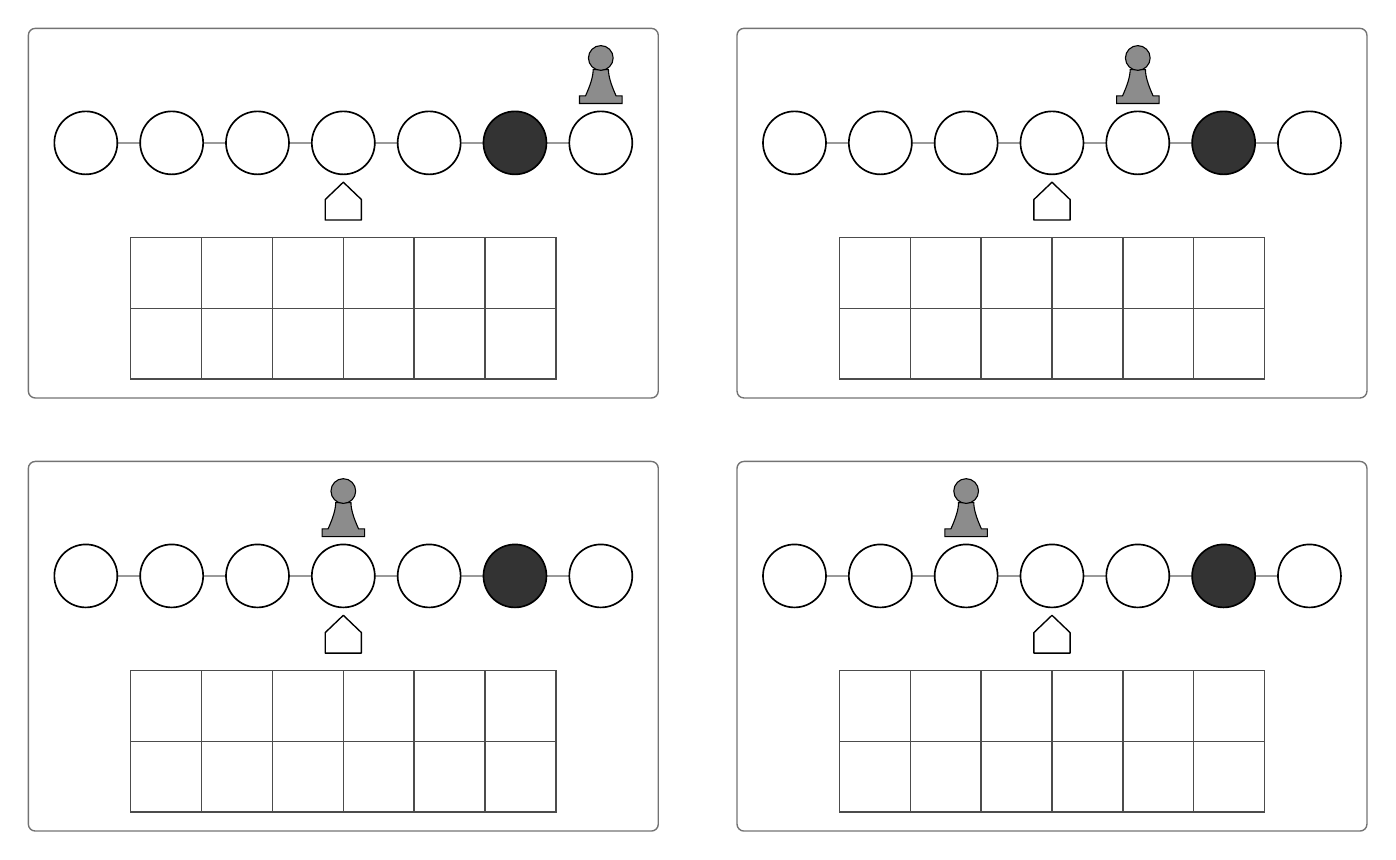
\begin{tikzpicture}[x=1mm, y=1mm]
\draw[line width=0.5pt, black!55, rounded corners=2.5] (-85.00,-32.40) rectangle (-5.00,14.54);
\draw[line width=0.9pt, black!40] (-77.70,0.00) -- (-12.30,0.00);
\draw[line width=0.6pt, fill=white] (-77.70,0.00) circle (4.0);
\draw[line width=0.6pt, fill=white] (-66.80,0.00) circle (4.0);
\draw[line width=0.6pt, fill=white] (-55.90,0.00) circle (4.0);
\draw[line width=0.6pt, fill=white] (-45.00,0.00) circle (4.0);
\draw[line width=0.6pt, fill=white] (-34.10,0.00) circle (4.0);
\draw[line width=0.6pt, fill=black!80] (-23.20,0.00) circle (4.0);
\draw[line width=0.6pt, fill=white] (-12.30,0.00) circle (4.0);
\draw[line width=0.4pt, fill=black!45] (-15.00,5.00) -- (-9.60,5.00) -- (-9.60,5.97) -- (-10.36,5.97) .. controls (-11.00,7.38) and (-11.33,8.46) .. (-11.33,9.32) -- (-13.27,9.32) .. controls (-13.27,8.46) and (-13.60,7.38) .. (-14.24,5.97) -- (-15.00,5.97) -- cycle;
\draw[line width=0.4pt, fill=black!45] (-12.30,10.78) circle (1.57);
\draw[line width=0.5pt, line join=round] (-45.00,-5.00) -- (-42.70,-7.20) -- (-42.70,-9.80) -- (-47.30,-9.80) -- (-47.30,-7.20) -- cycle;
\draw[line width=0.5pt, black!70] (-72.00,-21.00) rectangle (-63.00,-12.00);
\draw[line width=0.5pt, black!70] (-63.00,-21.00) rectangle (-54.00,-12.00);
\draw[line width=0.5pt, black!70] (-54.00,-21.00) rectangle (-45.00,-12.00);
\draw[line width=0.5pt, black!70] (-45.00,-21.00) rectangle (-36.00,-12.00);
\draw[line width=0.5pt, black!70] (-36.00,-21.00) rectangle (-27.00,-12.00);
\draw[line width=0.5pt, black!70] (-27.00,-21.00) rectangle (-18.00,-12.00);
\draw[line width=0.5pt, black!70] (-72.00,-30.00) rectangle (-63.00,-21.00);
\draw[line width=0.5pt, black!70] (-63.00,-30.00) rectangle (-54.00,-21.00);
\draw[line width=0.5pt, black!70] (-54.00,-30.00) rectangle (-45.00,-21.00);
\draw[line width=0.5pt, black!70] (-45.00,-30.00) rectangle (-36.00,-21.00);
\draw[line width=0.5pt, black!70] (-36.00,-30.00) rectangle (-27.00,-21.00);
\draw[line width=0.5pt, black!70] (-27.00,-30.00) rectangle (-18.00,-21.00);
\draw[line width=0.5pt, black!55, rounded corners=2.5] (5.00,-32.40) rectangle (85.00,14.54);
\draw[line width=0.9pt, black!40] (12.30,0.00) -- (77.70,0.00);
\draw[line width=0.6pt, fill=white] (12.30,0.00) circle (4.0);
\draw[line width=0.6pt, fill=white] (23.20,0.00) circle (4.0);
\draw[line width=0.6pt, fill=white] (34.10,0.00) circle (4.0);
\draw[line width=0.6pt, fill=white] (45.00,0.00) circle (4.0);
\draw[line width=0.6pt, fill=white] (55.90,0.00) circle (4.0);
\draw[line width=0.6pt, fill=black!80] (66.80,0.00) circle (4.0);
\draw[line width=0.6pt, fill=white] (77.70,0.00) circle (4.0);
\draw[line width=0.4pt, fill=black!45] (53.20,5.00) -- (58.60,5.00) -- (58.60,5.97) -- (57.84,5.97) .. controls (57.20,7.38) and (56.87,8.46) .. (56.87,9.32) -- (54.93,9.32) .. controls (54.93,8.46) and (54.60,7.38) .. (53.96,5.97) -- (53.20,5.97) -- cycle;
\draw[line width=0.4pt, fill=black!45] (55.90,10.78) circle (1.57);
\draw[line width=0.5pt, line join=round] (45.00,-5.00) -- (47.30,-7.20) -- (47.30,-9.80) -- (42.70,-9.80) -- (42.70,-7.20) -- cycle;
\draw[line width=0.5pt, black!70] (18.00,-21.00) rectangle (27.00,-12.00);
\draw[line width=0.5pt, black!70] (27.00,-21.00) rectangle (36.00,-12.00);
\draw[line width=0.5pt, black!70] (36.00,-21.00) rectangle (45.00,-12.00);
\draw[line width=0.5pt, black!70] (45.00,-21.00) rectangle (54.00,-12.00);
\draw[line width=0.5pt, black!70] (54.00,-21.00) rectangle (63.00,-12.00);
\draw[line width=0.5pt, black!70] (63.00,-21.00) rectangle (72.00,-12.00);
\draw[line width=0.5pt, black!70] (18.00,-30.00) rectangle (27.00,-21.00);
\draw[line width=0.5pt, black!70] (27.00,-30.00) rectangle (36.00,-21.00);
\draw[line width=0.5pt, black!70] (36.00,-30.00) rectangle (45.00,-21.00);
\draw[line width=0.5pt, black!70] (45.00,-30.00) rectangle (54.00,-21.00);
\draw[line width=0.5pt, black!70] (54.00,-30.00) rectangle (63.00,-21.00);
\draw[line width=0.5pt, black!70] (63.00,-30.00) rectangle (72.00,-21.00);
\draw[line width=0.5pt, black!55, rounded corners=2.5] (-85.00,-87.40) rectangle (-5.00,-40.46);
\draw[line width=0.9pt, black!40] (-77.70,-55.00) -- (-12.30,-55.00);
\draw[line width=0.6pt, fill=white] (-77.70,-55.00) circle (4.0);
\draw[line width=0.6pt, fill=white] (-66.80,-55.00) circle (4.0);
\draw[line width=0.6pt, fill=white] (-55.90,-55.00) circle (4.0);
\draw[line width=0.6pt, fill=white] (-45.00,-55.00) circle (4.0);
\draw[line width=0.6pt, fill=white] (-34.10,-55.00) circle (4.0);
\draw[line width=0.6pt, fill=black!80] (-23.20,-55.00) circle (4.0);
\draw[line width=0.6pt, fill=white] (-12.30,-55.00) circle (4.0);
\draw[line width=0.4pt, fill=black!45] (-47.70,-50.00) -- (-42.30,-50.00) -- (-42.30,-49.03) -- (-43.06,-49.03) .. controls (-43.70,-47.62) and (-44.03,-46.54) .. (-44.03,-45.68) -- (-45.97,-45.68) .. controls (-45.97,-46.54) and (-46.30,-47.62) .. (-46.94,-49.03) -- (-47.70,-49.03) -- cycle;
\draw[line width=0.4pt, fill=black!45] (-45.00,-44.22) circle (1.57);
\draw[line width=0.5pt, line join=round] (-45.00,-60.00) -- (-42.70,-62.20) -- (-42.70,-64.80) -- (-47.30,-64.80) -- (-47.30,-62.20) -- cycle;
\draw[line width=0.5pt, black!70] (-72.00,-76.00) rectangle (-63.00,-67.00);
\draw[line width=0.5pt, black!70] (-63.00,-76.00) rectangle (-54.00,-67.00);
\draw[line width=0.5pt, black!70] (-54.00,-76.00) rectangle (-45.00,-67.00);
\draw[line width=0.5pt, black!70] (-45.00,-76.00) rectangle (-36.00,-67.00);
\draw[line width=0.5pt, black!70] (-36.00,-76.00) rectangle (-27.00,-67.00);
\draw[line width=0.5pt, black!70] (-27.00,-76.00) rectangle (-18.00,-67.00);
\draw[line width=0.5pt, black!70] (-72.00,-85.00) rectangle (-63.00,-76.00);
\draw[line width=0.5pt, black!70] (-63.00,-85.00) rectangle (-54.00,-76.00);
\draw[line width=0.5pt, black!70] (-54.00,-85.00) rectangle (-45.00,-76.00);
\draw[line width=0.5pt, black!70] (-45.00,-85.00) rectangle (-36.00,-76.00);
\draw[line width=0.5pt, black!70] (-36.00,-85.00) rectangle (-27.00,-76.00);
\draw[line width=0.5pt, black!70] (-27.00,-85.00) rectangle (-18.00,-76.00);
\draw[line width=0.5pt, black!55, rounded corners=2.5] (5.00,-87.40) rectangle (85.00,-40.46);
\draw[line width=0.9pt, black!40] (12.30,-55.00) -- (77.70,-55.00);
\draw[line width=0.6pt, fill=white] (12.30,-55.00) circle (4.0);
\draw[line width=0.6pt, fill=white] (23.20,-55.00) circle (4.0);
\draw[line width=0.6pt, fill=white] (34.10,-55.00) circle (4.0);
\draw[line width=0.6pt, fill=white] (45.00,-55.00) circle (4.0);
\draw[line width=0.6pt, fill=white] (55.90,-55.00) circle (4.0);
\draw[line width=0.6pt, fill=black!80] (66.80,-55.00) circle (4.0);
\draw[line width=0.6pt, fill=white] (77.70,-55.00) circle (4.0);
\draw[line width=0.4pt, fill=black!45] (31.40,-50.00) -- (36.80,-50.00) -- (36.80,-49.03) -- (36.04,-49.03) .. controls (35.40,-47.62) and (35.07,-46.54) .. (35.07,-45.68) -- (33.13,-45.68) .. controls (33.13,-46.54) and (32.80,-47.62) .. (32.16,-49.03) -- (31.40,-49.03) -- cycle;
\draw[line width=0.4pt, fill=black!45] (34.10,-44.22) circle (1.57);
\draw[line width=0.5pt, line join=round] (45.00,-60.00) -- (47.30,-62.20) -- (47.30,-64.80) -- (42.70,-64.80) -- (42.70,-62.20) -- cycle;
\draw[line width=0.5pt, black!70] (18.00,-76.00) rectangle (27.00,-67.00);
\draw[line width=0.5pt, black!70] (27.00,-76.00) rectangle (36.00,-67.00);
\draw[line width=0.5pt, black!70] (36.00,-76.00) rectangle (45.00,-67.00);
\draw[line width=0.5pt, black!70] (45.00,-76.00) rectangle (54.00,-67.00);
\draw[line width=0.5pt, black!70] (54.00,-76.00) rectangle (63.00,-67.00);
\draw[line width=0.5pt, black!70] (63.00,-76.00) rectangle (72.00,-67.00);
\draw[line width=0.5pt, black!70] (18.00,-85.00) rectangle (27.00,-76.00);
\draw[line width=0.5pt, black!70] (27.00,-85.00) rectangle (36.00,-76.00);
\draw[line width=0.5pt, black!70] (36.00,-85.00) rectangle (45.00,-76.00);
\draw[line width=0.5pt, black!70] (45.00,-85.00) rectangle (54.00,-76.00);
\draw[line width=0.5pt, black!70] (54.00,-85.00) rectangle (63.00,-76.00);
\draw[line width=0.5pt, black!70] (63.00,-85.00) rectangle (72.00,-76.00);
\end{tikzpicture}}

\vfill
\centerline{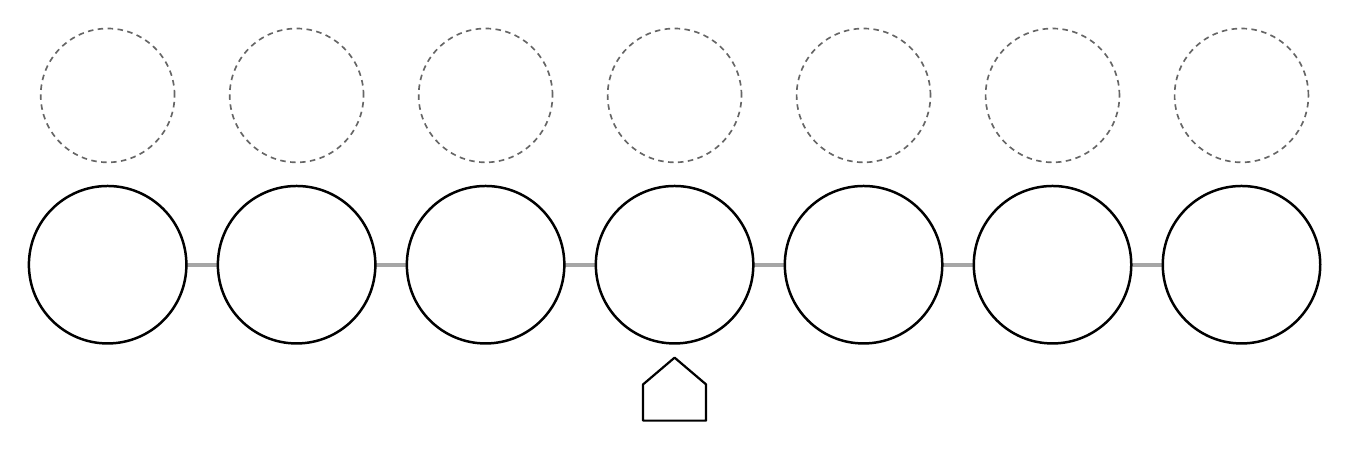
\begin{tikzpicture}[x=1mm, y=1mm]
\draw[line width=1.4pt, black!35] (-78.0,0) -- (78.0,0);
\draw[line width=0.9pt, fill=white] (-72.0,0) circle (10.0);
\draw[line width=0.6pt, black!60, dash pattern=on 2pt off 1.6pt] (-72.0,21.5) circle (8.5);
\draw[line width=0.9pt, fill=white] (-48.0,0) circle (10.0);
\draw[line width=0.6pt, black!60, dash pattern=on 2pt off 1.6pt] (-48.0,21.5) circle (8.5);
\draw[line width=0.9pt, fill=white] (-24.0,0) circle (10.0);
\draw[line width=0.6pt, black!60, dash pattern=on 2pt off 1.6pt] (-24.0,21.5) circle (8.5);
\draw[line width=0.9pt, fill=white] (0.0,0) circle (10.0);
\draw[line width=0.6pt, black!60, dash pattern=on 2pt off 1.6pt] (0.0,21.5) circle (8.5);
\draw[line width=0.9pt, fill=white] (24.0,0) circle (10.0);
\draw[line width=0.6pt, black!60, dash pattern=on 2pt off 1.6pt] (24.0,21.5) circle (8.5);
\draw[line width=0.9pt, fill=white] (48.0,0) circle (10.0);
\draw[line width=0.6pt, black!60, dash pattern=on 2pt off 1.6pt] (48.0,21.5) circle (8.5);
\draw[line width=0.9pt, fill=white] (72.0,0) circle (10.0);
\draw[line width=0.6pt, black!60, dash pattern=on 2pt off 1.6pt] (72.0,21.5) circle (8.5);
\draw[line width=0.8pt, line join=round] (0.00,-11.80) -- (4.00,-15.20) -- (4.00,-19.80) -- (-4.00,-19.80) -- (-4.00,-15.20) -- cycle;
\end{tikzpicture}}
\vspace*{2mm}
\newpage
\noindent\textbf{Problem 3:} Build each picture with as few moves as you can.

\vspace{5mm}\centerline{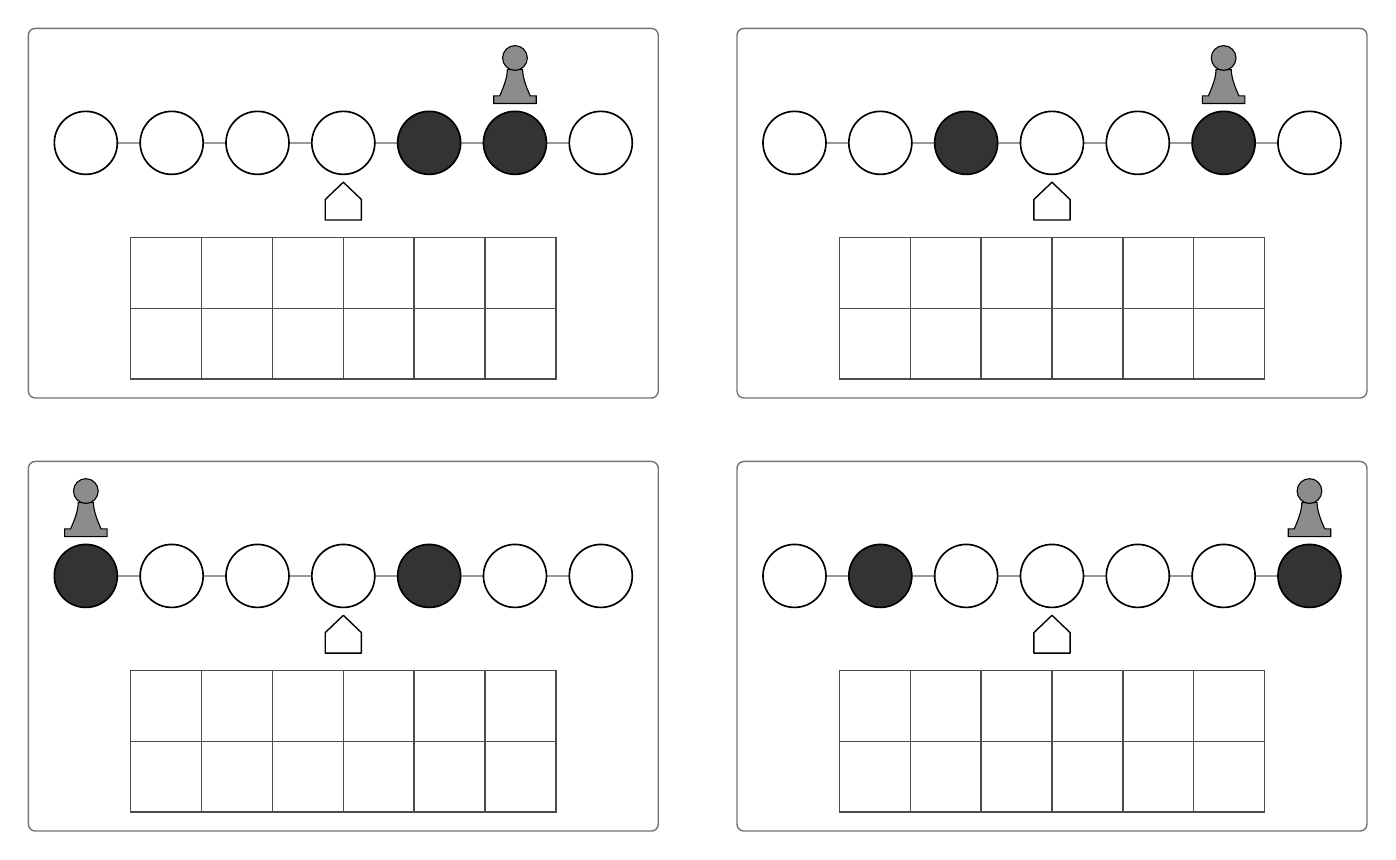
\begin{tikzpicture}[x=1mm, y=1mm]
\draw[line width=0.5pt, black!55, rounded corners=2.5] (-85.00,-32.40) rectangle (-5.00,14.54);
\draw[line width=0.9pt, black!40] (-77.70,0.00) -- (-12.30,0.00);
\draw[line width=0.6pt, fill=white] (-77.70,0.00) circle (4.0);
\draw[line width=0.6pt, fill=white] (-66.80,0.00) circle (4.0);
\draw[line width=0.6pt, fill=white] (-55.90,0.00) circle (4.0);
\draw[line width=0.6pt, fill=white] (-45.00,0.00) circle (4.0);
\draw[line width=0.6pt, fill=black!80] (-34.10,0.00) circle (4.0);
\draw[line width=0.6pt, fill=black!80] (-23.20,0.00) circle (4.0);
\draw[line width=0.6pt, fill=white] (-12.30,0.00) circle (4.0);
\draw[line width=0.4pt, fill=black!45] (-25.90,5.00) -- (-20.50,5.00) -- (-20.50,5.97) -- (-21.26,5.97) .. controls (-21.90,7.38) and (-22.23,8.46) .. (-22.23,9.32) -- (-24.17,9.32) .. controls (-24.17,8.46) and (-24.50,7.38) .. (-25.14,5.97) -- (-25.90,5.97) -- cycle;
\draw[line width=0.4pt, fill=black!45] (-23.20,10.78) circle (1.57);
\draw[line width=0.5pt, line join=round] (-45.00,-5.00) -- (-42.70,-7.20) -- (-42.70,-9.80) -- (-47.30,-9.80) -- (-47.30,-7.20) -- cycle;
\draw[line width=0.5pt, black!70] (-72.00,-21.00) rectangle (-63.00,-12.00);
\draw[line width=0.5pt, black!70] (-63.00,-21.00) rectangle (-54.00,-12.00);
\draw[line width=0.5pt, black!70] (-54.00,-21.00) rectangle (-45.00,-12.00);
\draw[line width=0.5pt, black!70] (-45.00,-21.00) rectangle (-36.00,-12.00);
\draw[line width=0.5pt, black!70] (-36.00,-21.00) rectangle (-27.00,-12.00);
\draw[line width=0.5pt, black!70] (-27.00,-21.00) rectangle (-18.00,-12.00);
\draw[line width=0.5pt, black!70] (-72.00,-30.00) rectangle (-63.00,-21.00);
\draw[line width=0.5pt, black!70] (-63.00,-30.00) rectangle (-54.00,-21.00);
\draw[line width=0.5pt, black!70] (-54.00,-30.00) rectangle (-45.00,-21.00);
\draw[line width=0.5pt, black!70] (-45.00,-30.00) rectangle (-36.00,-21.00);
\draw[line width=0.5pt, black!70] (-36.00,-30.00) rectangle (-27.00,-21.00);
\draw[line width=0.5pt, black!70] (-27.00,-30.00) rectangle (-18.00,-21.00);
\draw[line width=0.5pt, black!55, rounded corners=2.5] (5.00,-32.40) rectangle (85.00,14.54);
\draw[line width=0.9pt, black!40] (12.30,0.00) -- (77.70,0.00);
\draw[line width=0.6pt, fill=white] (12.30,0.00) circle (4.0);
\draw[line width=0.6pt, fill=white] (23.20,0.00) circle (4.0);
\draw[line width=0.6pt, fill=black!80] (34.10,0.00) circle (4.0);
\draw[line width=0.6pt, fill=white] (45.00,0.00) circle (4.0);
\draw[line width=0.6pt, fill=white] (55.90,0.00) circle (4.0);
\draw[line width=0.6pt, fill=black!80] (66.80,0.00) circle (4.0);
\draw[line width=0.6pt, fill=white] (77.70,0.00) circle (4.0);
\draw[line width=0.4pt, fill=black!45] (64.10,5.00) -- (69.50,5.00) -- (69.50,5.97) -- (68.74,5.97) .. controls (68.10,7.38) and (67.77,8.46) .. (67.77,9.32) -- (65.83,9.32) .. controls (65.83,8.46) and (65.50,7.38) .. (64.86,5.97) -- (64.10,5.97) -- cycle;
\draw[line width=0.4pt, fill=black!45] (66.80,10.78) circle (1.57);
\draw[line width=0.5pt, line join=round] (45.00,-5.00) -- (47.30,-7.20) -- (47.30,-9.80) -- (42.70,-9.80) -- (42.70,-7.20) -- cycle;
\draw[line width=0.5pt, black!70] (18.00,-21.00) rectangle (27.00,-12.00);
\draw[line width=0.5pt, black!70] (27.00,-21.00) rectangle (36.00,-12.00);
\draw[line width=0.5pt, black!70] (36.00,-21.00) rectangle (45.00,-12.00);
\draw[line width=0.5pt, black!70] (45.00,-21.00) rectangle (54.00,-12.00);
\draw[line width=0.5pt, black!70] (54.00,-21.00) rectangle (63.00,-12.00);
\draw[line width=0.5pt, black!70] (63.00,-21.00) rectangle (72.00,-12.00);
\draw[line width=0.5pt, black!70] (18.00,-30.00) rectangle (27.00,-21.00);
\draw[line width=0.5pt, black!70] (27.00,-30.00) rectangle (36.00,-21.00);
\draw[line width=0.5pt, black!70] (36.00,-30.00) rectangle (45.00,-21.00);
\draw[line width=0.5pt, black!70] (45.00,-30.00) rectangle (54.00,-21.00);
\draw[line width=0.5pt, black!70] (54.00,-30.00) rectangle (63.00,-21.00);
\draw[line width=0.5pt, black!70] (63.00,-30.00) rectangle (72.00,-21.00);
\draw[line width=0.5pt, black!55, rounded corners=2.5] (-85.00,-87.40) rectangle (-5.00,-40.46);
\draw[line width=0.9pt, black!40] (-77.70,-55.00) -- (-12.30,-55.00);
\draw[line width=0.6pt, fill=black!80] (-77.70,-55.00) circle (4.0);
\draw[line width=0.6pt, fill=white] (-66.80,-55.00) circle (4.0);
\draw[line width=0.6pt, fill=white] (-55.90,-55.00) circle (4.0);
\draw[line width=0.6pt, fill=white] (-45.00,-55.00) circle (4.0);
\draw[line width=0.6pt, fill=black!80] (-34.10,-55.00) circle (4.0);
\draw[line width=0.6pt, fill=white] (-23.20,-55.00) circle (4.0);
\draw[line width=0.6pt, fill=white] (-12.30,-55.00) circle (4.0);
\draw[line width=0.4pt, fill=black!45] (-80.40,-50.00) -- (-75.00,-50.00) -- (-75.00,-49.03) -- (-75.76,-49.03) .. controls (-76.40,-47.62) and (-76.73,-46.54) .. (-76.73,-45.68) -- (-78.67,-45.68) .. controls (-78.67,-46.54) and (-79.00,-47.62) .. (-79.64,-49.03) -- (-80.40,-49.03) -- cycle;
\draw[line width=0.4pt, fill=black!45] (-77.70,-44.22) circle (1.57);
\draw[line width=0.5pt, line join=round] (-45.00,-60.00) -- (-42.70,-62.20) -- (-42.70,-64.80) -- (-47.30,-64.80) -- (-47.30,-62.20) -- cycle;
\draw[line width=0.5pt, black!70] (-72.00,-76.00) rectangle (-63.00,-67.00);
\draw[line width=0.5pt, black!70] (-63.00,-76.00) rectangle (-54.00,-67.00);
\draw[line width=0.5pt, black!70] (-54.00,-76.00) rectangle (-45.00,-67.00);
\draw[line width=0.5pt, black!70] (-45.00,-76.00) rectangle (-36.00,-67.00);
\draw[line width=0.5pt, black!70] (-36.00,-76.00) rectangle (-27.00,-67.00);
\draw[line width=0.5pt, black!70] (-27.00,-76.00) rectangle (-18.00,-67.00);
\draw[line width=0.5pt, black!70] (-72.00,-85.00) rectangle (-63.00,-76.00);
\draw[line width=0.5pt, black!70] (-63.00,-85.00) rectangle (-54.00,-76.00);
\draw[line width=0.5pt, black!70] (-54.00,-85.00) rectangle (-45.00,-76.00);
\draw[line width=0.5pt, black!70] (-45.00,-85.00) rectangle (-36.00,-76.00);
\draw[line width=0.5pt, black!70] (-36.00,-85.00) rectangle (-27.00,-76.00);
\draw[line width=0.5pt, black!70] (-27.00,-85.00) rectangle (-18.00,-76.00);
\draw[line width=0.5pt, black!55, rounded corners=2.5] (5.00,-87.40) rectangle (85.00,-40.46);
\draw[line width=0.9pt, black!40] (12.30,-55.00) -- (77.70,-55.00);
\draw[line width=0.6pt, fill=white] (12.30,-55.00) circle (4.0);
\draw[line width=0.6pt, fill=black!80] (23.20,-55.00) circle (4.0);
\draw[line width=0.6pt, fill=white] (34.10,-55.00) circle (4.0);
\draw[line width=0.6pt, fill=white] (45.00,-55.00) circle (4.0);
\draw[line width=0.6pt, fill=white] (55.90,-55.00) circle (4.0);
\draw[line width=0.6pt, fill=white] (66.80,-55.00) circle (4.0);
\draw[line width=0.6pt, fill=black!80] (77.70,-55.00) circle (4.0);
\draw[line width=0.4pt, fill=black!45] (75.00,-50.00) -- (80.40,-50.00) -- (80.40,-49.03) -- (79.64,-49.03) .. controls (79.00,-47.62) and (78.67,-46.54) .. (78.67,-45.68) -- (76.73,-45.68) .. controls (76.73,-46.54) and (76.40,-47.62) .. (75.76,-49.03) -- (75.00,-49.03) -- cycle;
\draw[line width=0.4pt, fill=black!45] (77.70,-44.22) circle (1.57);
\draw[line width=0.5pt, line join=round] (45.00,-60.00) -- (47.30,-62.20) -- (47.30,-64.80) -- (42.70,-64.80) -- (42.70,-62.20) -- cycle;
\draw[line width=0.5pt, black!70] (18.00,-76.00) rectangle (27.00,-67.00);
\draw[line width=0.5pt, black!70] (27.00,-76.00) rectangle (36.00,-67.00);
\draw[line width=0.5pt, black!70] (36.00,-76.00) rectangle (45.00,-67.00);
\draw[line width=0.5pt, black!70] (45.00,-76.00) rectangle (54.00,-67.00);
\draw[line width=0.5pt, black!70] (54.00,-76.00) rectangle (63.00,-67.00);
\draw[line width=0.5pt, black!70] (63.00,-76.00) rectangle (72.00,-67.00);
\draw[line width=0.5pt, black!70] (18.00,-85.00) rectangle (27.00,-76.00);
\draw[line width=0.5pt, black!70] (27.00,-85.00) rectangle (36.00,-76.00);
\draw[line width=0.5pt, black!70] (36.00,-85.00) rectangle (45.00,-76.00);
\draw[line width=0.5pt, black!70] (45.00,-85.00) rectangle (54.00,-76.00);
\draw[line width=0.5pt, black!70] (54.00,-85.00) rectangle (63.00,-76.00);
\draw[line width=0.5pt, black!70] (63.00,-85.00) rectangle (72.00,-76.00);
\end{tikzpicture}}

\vfill
\centerline{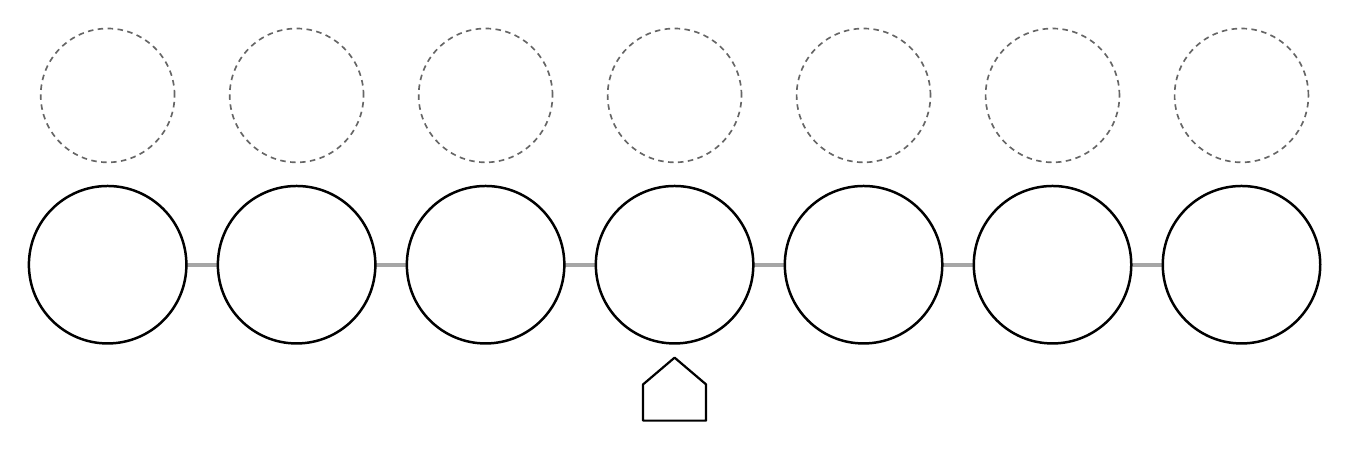
\begin{tikzpicture}[x=1mm, y=1mm]
\draw[line width=1.4pt, black!35] (-78.0,0) -- (78.0,0);
\draw[line width=0.9pt, fill=white] (-72.0,0) circle (10.0);
\draw[line width=0.6pt, black!60, dash pattern=on 2pt off 1.6pt] (-72.0,21.5) circle (8.5);
\draw[line width=0.9pt, fill=white] (-48.0,0) circle (10.0);
\draw[line width=0.6pt, black!60, dash pattern=on 2pt off 1.6pt] (-48.0,21.5) circle (8.5);
\draw[line width=0.9pt, fill=white] (-24.0,0) circle (10.0);
\draw[line width=0.6pt, black!60, dash pattern=on 2pt off 1.6pt] (-24.0,21.5) circle (8.5);
\draw[line width=0.9pt, fill=white] (0.0,0) circle (10.0);
\draw[line width=0.6pt, black!60, dash pattern=on 2pt off 1.6pt] (0.0,21.5) circle (8.5);
\draw[line width=0.9pt, fill=white] (24.0,0) circle (10.0);
\draw[line width=0.6pt, black!60, dash pattern=on 2pt off 1.6pt] (24.0,21.5) circle (8.5);
\draw[line width=0.9pt, fill=white] (48.0,0) circle (10.0);
\draw[line width=0.6pt, black!60, dash pattern=on 2pt off 1.6pt] (48.0,21.5) circle (8.5);
\draw[line width=0.9pt, fill=white] (72.0,0) circle (10.0);
\draw[line width=0.6pt, black!60, dash pattern=on 2pt off 1.6pt] (72.0,21.5) circle (8.5);
\draw[line width=0.8pt, line join=round] (0.00,-11.80) -- (4.00,-15.20) -- (4.00,-19.80) -- (-4.00,-19.80) -- (-4.00,-15.20) -- cycle;
\end{tikzpicture}}
\vspace*{2mm}
\newpage
\noindent\textbf{Problem 4:} Build each picture with as few moves as you can.

\vspace{5mm}\centerline{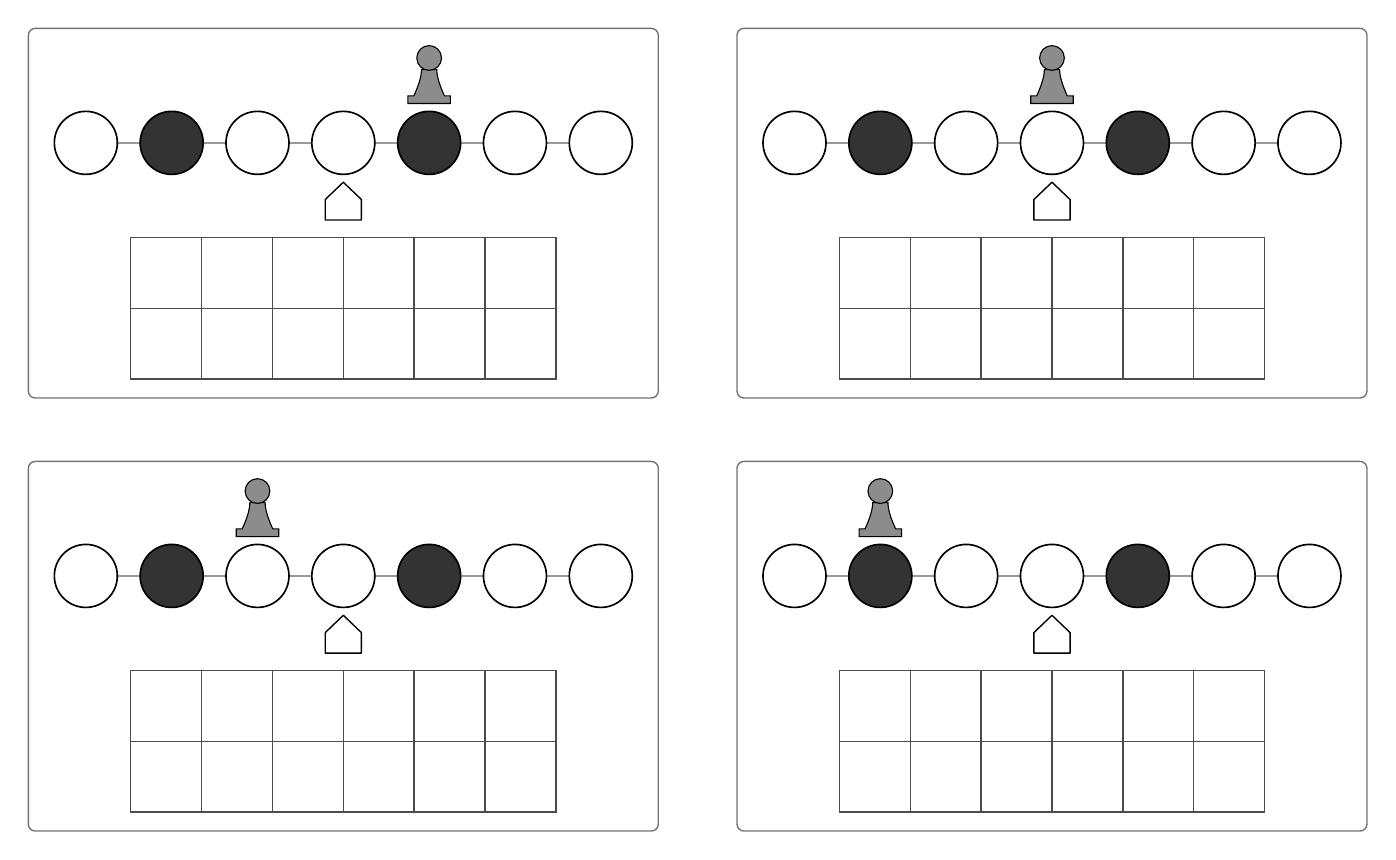
\begin{tikzpicture}[x=1mm, y=1mm]
\draw[line width=0.5pt, black!55, rounded corners=2.5] (-85.00,-32.40) rectangle (-5.00,14.54);
\draw[line width=0.9pt, black!40] (-77.70,0.00) -- (-12.30,0.00);
\draw[line width=0.6pt, fill=white] (-77.70,0.00) circle (4.0);
\draw[line width=0.6pt, fill=black!80] (-66.80,0.00) circle (4.0);
\draw[line width=0.6pt, fill=white] (-55.90,0.00) circle (4.0);
\draw[line width=0.6pt, fill=white] (-45.00,0.00) circle (4.0);
\draw[line width=0.6pt, fill=black!80] (-34.10,0.00) circle (4.0);
\draw[line width=0.6pt, fill=white] (-23.20,0.00) circle (4.0);
\draw[line width=0.6pt, fill=white] (-12.30,0.00) circle (4.0);
\draw[line width=0.4pt, fill=black!45] (-36.80,5.00) -- (-31.40,5.00) -- (-31.40,5.97) -- (-32.16,5.97) .. controls (-32.80,7.38) and (-33.13,8.46) .. (-33.13,9.32) -- (-35.07,9.32) .. controls (-35.07,8.46) and (-35.40,7.38) .. (-36.04,5.97) -- (-36.80,5.97) -- cycle;
\draw[line width=0.4pt, fill=black!45] (-34.10,10.78) circle (1.57);
\draw[line width=0.5pt, line join=round] (-45.00,-5.00) -- (-42.70,-7.20) -- (-42.70,-9.80) -- (-47.30,-9.80) -- (-47.30,-7.20) -- cycle;
\draw[line width=0.5pt, black!70] (-72.00,-21.00) rectangle (-63.00,-12.00);
\draw[line width=0.5pt, black!70] (-63.00,-21.00) rectangle (-54.00,-12.00);
\draw[line width=0.5pt, black!70] (-54.00,-21.00) rectangle (-45.00,-12.00);
\draw[line width=0.5pt, black!70] (-45.00,-21.00) rectangle (-36.00,-12.00);
\draw[line width=0.5pt, black!70] (-36.00,-21.00) rectangle (-27.00,-12.00);
\draw[line width=0.5pt, black!70] (-27.00,-21.00) rectangle (-18.00,-12.00);
\draw[line width=0.5pt, black!70] (-72.00,-30.00) rectangle (-63.00,-21.00);
\draw[line width=0.5pt, black!70] (-63.00,-30.00) rectangle (-54.00,-21.00);
\draw[line width=0.5pt, black!70] (-54.00,-30.00) rectangle (-45.00,-21.00);
\draw[line width=0.5pt, black!70] (-45.00,-30.00) rectangle (-36.00,-21.00);
\draw[line width=0.5pt, black!70] (-36.00,-30.00) rectangle (-27.00,-21.00);
\draw[line width=0.5pt, black!70] (-27.00,-30.00) rectangle (-18.00,-21.00);
\draw[line width=0.5pt, black!55, rounded corners=2.5] (5.00,-32.40) rectangle (85.00,14.54);
\draw[line width=0.9pt, black!40] (12.30,0.00) -- (77.70,0.00);
\draw[line width=0.6pt, fill=white] (12.30,0.00) circle (4.0);
\draw[line width=0.6pt, fill=black!80] (23.20,0.00) circle (4.0);
\draw[line width=0.6pt, fill=white] (34.10,0.00) circle (4.0);
\draw[line width=0.6pt, fill=white] (45.00,0.00) circle (4.0);
\draw[line width=0.6pt, fill=black!80] (55.90,0.00) circle (4.0);
\draw[line width=0.6pt, fill=white] (66.80,0.00) circle (4.0);
\draw[line width=0.6pt, fill=white] (77.70,0.00) circle (4.0);
\draw[line width=0.4pt, fill=black!45] (42.30,5.00) -- (47.70,5.00) -- (47.70,5.97) -- (46.94,5.97) .. controls (46.30,7.38) and (45.97,8.46) .. (45.97,9.32) -- (44.03,9.32) .. controls (44.03,8.46) and (43.70,7.38) .. (43.06,5.97) -- (42.30,5.97) -- cycle;
\draw[line width=0.4pt, fill=black!45] (45.00,10.78) circle (1.57);
\draw[line width=0.5pt, line join=round] (45.00,-5.00) -- (47.30,-7.20) -- (47.30,-9.80) -- (42.70,-9.80) -- (42.70,-7.20) -- cycle;
\draw[line width=0.5pt, black!70] (18.00,-21.00) rectangle (27.00,-12.00);
\draw[line width=0.5pt, black!70] (27.00,-21.00) rectangle (36.00,-12.00);
\draw[line width=0.5pt, black!70] (36.00,-21.00) rectangle (45.00,-12.00);
\draw[line width=0.5pt, black!70] (45.00,-21.00) rectangle (54.00,-12.00);
\draw[line width=0.5pt, black!70] (54.00,-21.00) rectangle (63.00,-12.00);
\draw[line width=0.5pt, black!70] (63.00,-21.00) rectangle (72.00,-12.00);
\draw[line width=0.5pt, black!70] (18.00,-30.00) rectangle (27.00,-21.00);
\draw[line width=0.5pt, black!70] (27.00,-30.00) rectangle (36.00,-21.00);
\draw[line width=0.5pt, black!70] (36.00,-30.00) rectangle (45.00,-21.00);
\draw[line width=0.5pt, black!70] (45.00,-30.00) rectangle (54.00,-21.00);
\draw[line width=0.5pt, black!70] (54.00,-30.00) rectangle (63.00,-21.00);
\draw[line width=0.5pt, black!70] (63.00,-30.00) rectangle (72.00,-21.00);
\draw[line width=0.5pt, black!55, rounded corners=2.5] (-85.00,-87.40) rectangle (-5.00,-40.46);
\draw[line width=0.9pt, black!40] (-77.70,-55.00) -- (-12.30,-55.00);
\draw[line width=0.6pt, fill=white] (-77.70,-55.00) circle (4.0);
\draw[line width=0.6pt, fill=black!80] (-66.80,-55.00) circle (4.0);
\draw[line width=0.6pt, fill=white] (-55.90,-55.00) circle (4.0);
\draw[line width=0.6pt, fill=white] (-45.00,-55.00) circle (4.0);
\draw[line width=0.6pt, fill=black!80] (-34.10,-55.00) circle (4.0);
\draw[line width=0.6pt, fill=white] (-23.20,-55.00) circle (4.0);
\draw[line width=0.6pt, fill=white] (-12.30,-55.00) circle (4.0);
\draw[line width=0.4pt, fill=black!45] (-58.60,-50.00) -- (-53.20,-50.00) -- (-53.20,-49.03) -- (-53.96,-49.03) .. controls (-54.60,-47.62) and (-54.93,-46.54) .. (-54.93,-45.68) -- (-56.87,-45.68) .. controls (-56.87,-46.54) and (-57.20,-47.62) .. (-57.84,-49.03) -- (-58.60,-49.03) -- cycle;
\draw[line width=0.4pt, fill=black!45] (-55.90,-44.22) circle (1.57);
\draw[line width=0.5pt, line join=round] (-45.00,-60.00) -- (-42.70,-62.20) -- (-42.70,-64.80) -- (-47.30,-64.80) -- (-47.30,-62.20) -- cycle;
\draw[line width=0.5pt, black!70] (-72.00,-76.00) rectangle (-63.00,-67.00);
\draw[line width=0.5pt, black!70] (-63.00,-76.00) rectangle (-54.00,-67.00);
\draw[line width=0.5pt, black!70] (-54.00,-76.00) rectangle (-45.00,-67.00);
\draw[line width=0.5pt, black!70] (-45.00,-76.00) rectangle (-36.00,-67.00);
\draw[line width=0.5pt, black!70] (-36.00,-76.00) rectangle (-27.00,-67.00);
\draw[line width=0.5pt, black!70] (-27.00,-76.00) rectangle (-18.00,-67.00);
\draw[line width=0.5pt, black!70] (-72.00,-85.00) rectangle (-63.00,-76.00);
\draw[line width=0.5pt, black!70] (-63.00,-85.00) rectangle (-54.00,-76.00);
\draw[line width=0.5pt, black!70] (-54.00,-85.00) rectangle (-45.00,-76.00);
\draw[line width=0.5pt, black!70] (-45.00,-85.00) rectangle (-36.00,-76.00);
\draw[line width=0.5pt, black!70] (-36.00,-85.00) rectangle (-27.00,-76.00);
\draw[line width=0.5pt, black!70] (-27.00,-85.00) rectangle (-18.00,-76.00);
\draw[line width=0.5pt, black!55, rounded corners=2.5] (5.00,-87.40) rectangle (85.00,-40.46);
\draw[line width=0.9pt, black!40] (12.30,-55.00) -- (77.70,-55.00);
\draw[line width=0.6pt, fill=white] (12.30,-55.00) circle (4.0);
\draw[line width=0.6pt, fill=black!80] (23.20,-55.00) circle (4.0);
\draw[line width=0.6pt, fill=white] (34.10,-55.00) circle (4.0);
\draw[line width=0.6pt, fill=white] (45.00,-55.00) circle (4.0);
\draw[line width=0.6pt, fill=black!80] (55.90,-55.00) circle (4.0);
\draw[line width=0.6pt, fill=white] (66.80,-55.00) circle (4.0);
\draw[line width=0.6pt, fill=white] (77.70,-55.00) circle (4.0);
\draw[line width=0.4pt, fill=black!45] (20.50,-50.00) -- (25.90,-50.00) -- (25.90,-49.03) -- (25.14,-49.03) .. controls (24.50,-47.62) and (24.17,-46.54) .. (24.17,-45.68) -- (22.23,-45.68) .. controls (22.23,-46.54) and (21.90,-47.62) .. (21.26,-49.03) -- (20.50,-49.03) -- cycle;
\draw[line width=0.4pt, fill=black!45] (23.20,-44.22) circle (1.57);
\draw[line width=0.5pt, line join=round] (45.00,-60.00) -- (47.30,-62.20) -- (47.30,-64.80) -- (42.70,-64.80) -- (42.70,-62.20) -- cycle;
\draw[line width=0.5pt, black!70] (18.00,-76.00) rectangle (27.00,-67.00);
\draw[line width=0.5pt, black!70] (27.00,-76.00) rectangle (36.00,-67.00);
\draw[line width=0.5pt, black!70] (36.00,-76.00) rectangle (45.00,-67.00);
\draw[line width=0.5pt, black!70] (45.00,-76.00) rectangle (54.00,-67.00);
\draw[line width=0.5pt, black!70] (54.00,-76.00) rectangle (63.00,-67.00);
\draw[line width=0.5pt, black!70] (63.00,-76.00) rectangle (72.00,-67.00);
\draw[line width=0.5pt, black!70] (18.00,-85.00) rectangle (27.00,-76.00);
\draw[line width=0.5pt, black!70] (27.00,-85.00) rectangle (36.00,-76.00);
\draw[line width=0.5pt, black!70] (36.00,-85.00) rectangle (45.00,-76.00);
\draw[line width=0.5pt, black!70] (45.00,-85.00) rectangle (54.00,-76.00);
\draw[line width=0.5pt, black!70] (54.00,-85.00) rectangle (63.00,-76.00);
\draw[line width=0.5pt, black!70] (63.00,-85.00) rectangle (72.00,-76.00);
\end{tikzpicture}}

\vfill
\centerline{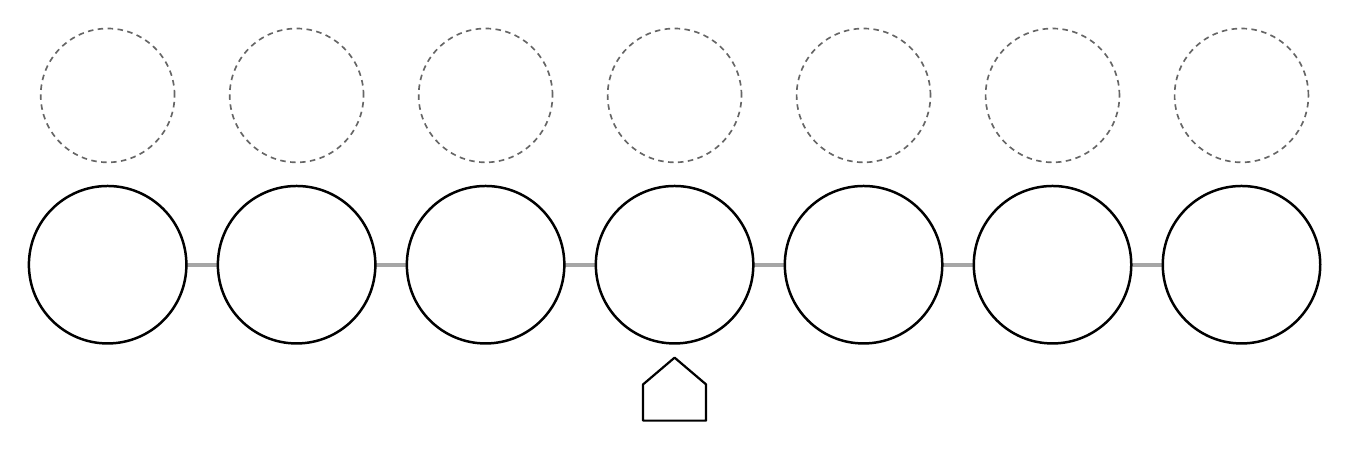
\begin{tikzpicture}[x=1mm, y=1mm]
\draw[line width=1.4pt, black!35] (-78.0,0) -- (78.0,0);
\draw[line width=0.9pt, fill=white] (-72.0,0) circle (10.0);
\draw[line width=0.6pt, black!60, dash pattern=on 2pt off 1.6pt] (-72.0,21.5) circle (8.5);
\draw[line width=0.9pt, fill=white] (-48.0,0) circle (10.0);
\draw[line width=0.6pt, black!60, dash pattern=on 2pt off 1.6pt] (-48.0,21.5) circle (8.5);
\draw[line width=0.9pt, fill=white] (-24.0,0) circle (10.0);
\draw[line width=0.6pt, black!60, dash pattern=on 2pt off 1.6pt] (-24.0,21.5) circle (8.5);
\draw[line width=0.9pt, fill=white] (0.0,0) circle (10.0);
\draw[line width=0.6pt, black!60, dash pattern=on 2pt off 1.6pt] (0.0,21.5) circle (8.5);
\draw[line width=0.9pt, fill=white] (24.0,0) circle (10.0);
\draw[line width=0.6pt, black!60, dash pattern=on 2pt off 1.6pt] (24.0,21.5) circle (8.5);
\draw[line width=0.9pt, fill=white] (48.0,0) circle (10.0);
\draw[line width=0.6pt, black!60, dash pattern=on 2pt off 1.6pt] (48.0,21.5) circle (8.5);
\draw[line width=0.9pt, fill=white] (72.0,0) circle (10.0);
\draw[line width=0.6pt, black!60, dash pattern=on 2pt off 1.6pt] (72.0,21.5) circle (8.5);
\draw[line width=0.8pt, line join=round] (0.00,-11.80) -- (4.00,-15.20) -- (4.00,-19.80) -- (-4.00,-19.80) -- (-4.00,-15.20) -- cycle;
\end{tikzpicture}}
\vspace*{2mm}
\newpage
\noindent\textbf{Problem 5:} Find every way to build each picture with the fewest moves. Draw each way in a row of squares, with a dot for each flip and an arrow for each step. Explain why there is no quicker way.

\vspace{4mm}\centerline{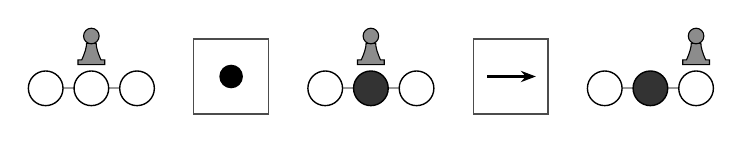
\begin{tikzpicture}[x=1mm, y=1mm]
\draw[line width=0.7pt, black!40] (-5.80,0.00) -- (5.80,0.00);
\draw[line width=0.5pt, fill=white] (-5.80,0.00) circle (2.2);
\draw[line width=0.5pt, fill=white] (0.00,0.00) circle (2.2);
\draw[line width=0.5pt, fill=white] (5.80,0.00) circle (2.2);
\draw[line width=0.4pt, fill=black!45] (-1.70,3.00) -- (1.70,3.00) -- (1.70,3.61) -- (1.22,3.61) .. controls (0.82,4.50) and (0.61,5.18) .. (0.61,5.72) -- (-0.61,5.72) .. controls (-0.61,5.18) and (-0.82,4.50) .. (-1.22,3.61) -- (-1.70,3.61) -- cycle;
\draw[line width=0.4pt, fill=black!45] (0.00,6.64) circle (0.99);
\draw[line width=0.5pt, black!70] (13.00,-3.25) rectangle (22.50,6.25);
\fill (17.75,1.50) circle (1.5);
\draw[line width=0.7pt, black!40] (29.70,0.00) -- (41.30,0.00);
\draw[line width=0.5pt, fill=white] (29.70,0.00) circle (2.2);
\draw[line width=0.5pt, fill=black!80] (35.50,0.00) circle (2.2);
\draw[line width=0.5pt, fill=white] (41.30,0.00) circle (2.2);
\draw[line width=0.4pt, fill=black!45] (33.80,3.00) -- (37.20,3.00) -- (37.20,3.61) -- (36.72,3.61) .. controls (36.32,4.50) and (36.11,5.18) .. (36.11,5.72) -- (34.89,5.72) .. controls (34.89,5.18) and (34.68,4.50) .. (34.28,3.61) -- (33.80,3.61) -- cycle;
\draw[line width=0.4pt, fill=black!45] (35.50,6.64) circle (0.99);
\draw[line width=0.5pt, black!70] (48.50,-3.25) rectangle (58.00,6.25);
\draw[-{Stealth[length=1.9mm]}, line width=0.9pt] (50.25,1.50) -- (56.45,1.50);
\draw[line width=0.7pt, black!40] (65.20,0.00) -- (76.80,0.00);
\draw[line width=0.5pt, fill=white] (65.20,0.00) circle (2.2);
\draw[line width=0.5pt, fill=black!80] (71.00,0.00) circle (2.2);
\draw[line width=0.5pt, fill=white] (76.80,0.00) circle (2.2);
\draw[line width=0.4pt, fill=black!45] (75.10,3.00) -- (78.50,3.00) -- (78.50,3.61) -- (78.02,3.61) .. controls (77.62,4.50) and (77.41,5.18) .. (77.41,5.72) -- (76.19,5.72) .. controls (76.19,5.18) and (75.98,4.50) .. (75.58,3.61) -- (75.10,3.61) -- cycle;
\draw[line width=0.4pt, fill=black!45] (76.80,6.64) circle (0.99);
\end{tikzpicture}}

\vspace{7mm}\centerline{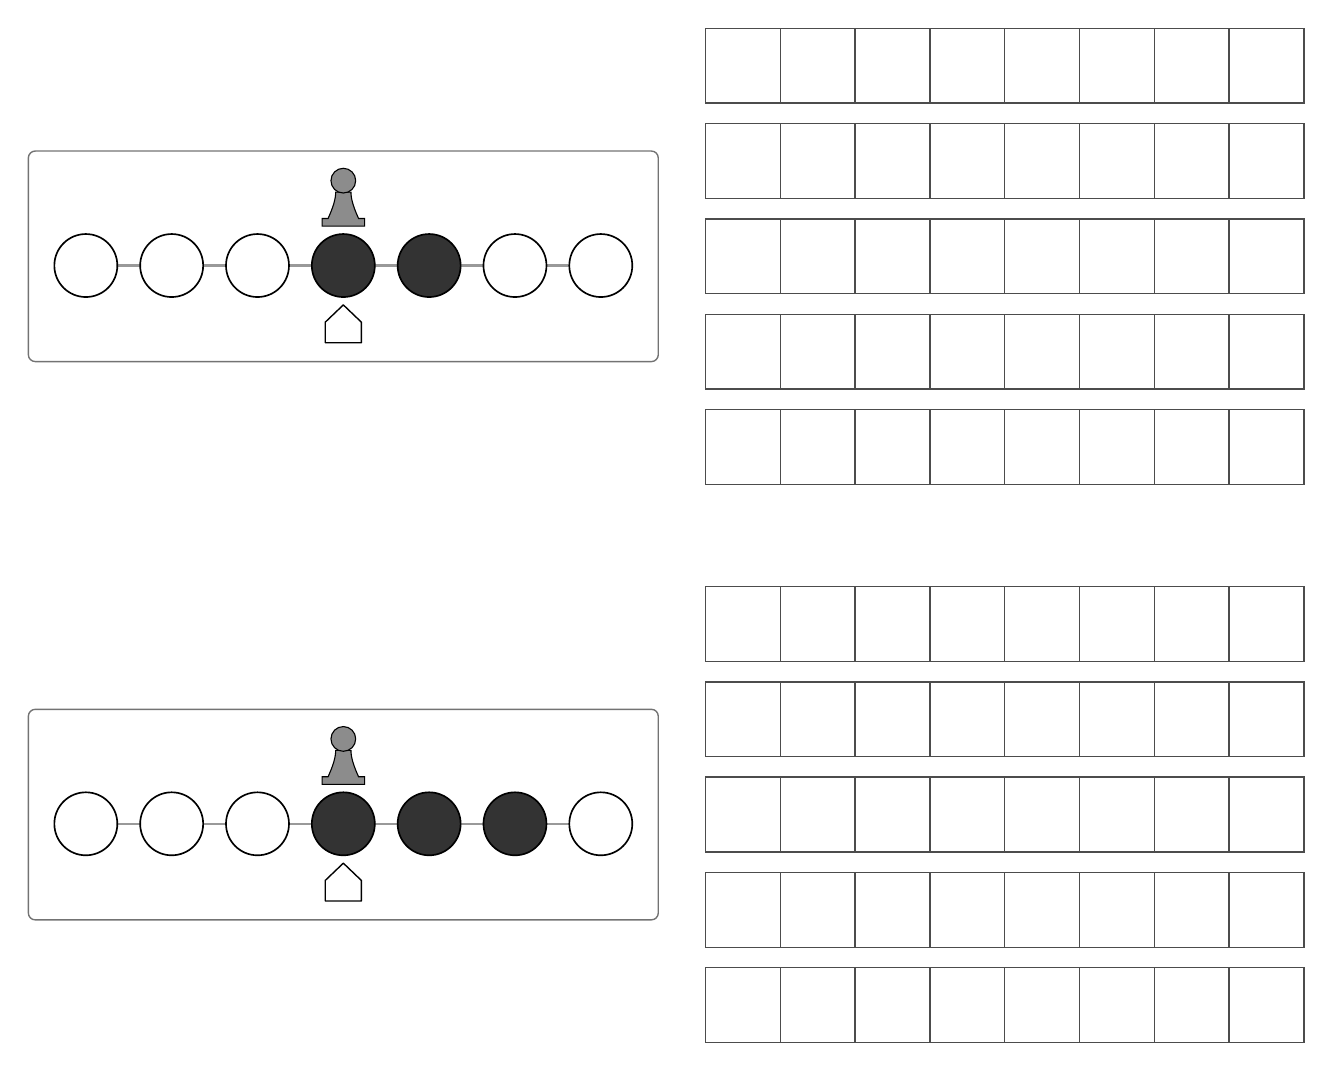
\begin{tikzpicture}[x=1mm, y=1mm]
\draw[line width=0.5pt, black!55, rounded corners=2.5] (-83.00,-42.32) rectangle (-3.00,-15.58);
\draw[line width=0.9pt, black!40] (-75.70,-30.12) -- (-10.30,-30.12);
\draw[line width=0.6pt, fill=white] (-75.70,-30.12) circle (4.0);
\draw[line width=0.6pt, fill=white] (-64.80,-30.12) circle (4.0);
\draw[line width=0.6pt, fill=white] (-53.90,-30.12) circle (4.0);
\draw[line width=0.6pt, fill=black!80] (-43.00,-30.12) circle (4.0);
\draw[line width=0.6pt, fill=black!80] (-32.10,-30.12) circle (4.0);
\draw[line width=0.6pt, fill=white] (-21.20,-30.12) circle (4.0);
\draw[line width=0.6pt, fill=white] (-10.30,-30.12) circle (4.0);
\draw[line width=0.4pt, fill=black!45] (-45.70,-25.12) -- (-40.30,-25.12) -- (-40.30,-24.15) -- (-41.06,-24.15) .. controls (-41.70,-22.75) and (-42.03,-21.67) .. (-42.03,-20.80) -- (-43.97,-20.80) .. controls (-43.97,-21.67) and (-44.30,-22.75) .. (-44.94,-24.15) -- (-45.70,-24.15) -- cycle;
\draw[line width=0.4pt, fill=black!45] (-43.00,-19.34) circle (1.57);
\draw[line width=0.5pt, line join=round] (-43.00,-35.12) -- (-40.70,-37.32) -- (-40.70,-39.92) -- (-45.30,-39.92) -- (-45.30,-37.32) -- cycle;
\draw[line width=0.5pt, black!70] (3.00,-9.50) rectangle (12.50,0.00);
\draw[line width=0.5pt, black!70] (12.50,-9.50) rectangle (22.00,0.00);
\draw[line width=0.5pt, black!70] (22.00,-9.50) rectangle (31.50,0.00);
\draw[line width=0.5pt, black!70] (31.50,-9.50) rectangle (41.00,0.00);
\draw[line width=0.5pt, black!70] (41.00,-9.50) rectangle (50.50,0.00);
\draw[line width=0.5pt, black!70] (50.50,-9.50) rectangle (60.00,0.00);
\draw[line width=0.5pt, black!70] (60.00,-9.50) rectangle (69.50,0.00);
\draw[line width=0.5pt, black!70] (69.50,-9.50) rectangle (79.00,0.00);
\draw[line width=0.5pt, black!70] (3.00,-21.60) rectangle (12.50,-12.10);
\draw[line width=0.5pt, black!70] (12.50,-21.60) rectangle (22.00,-12.10);
\draw[line width=0.5pt, black!70] (22.00,-21.60) rectangle (31.50,-12.10);
\draw[line width=0.5pt, black!70] (31.50,-21.60) rectangle (41.00,-12.10);
\draw[line width=0.5pt, black!70] (41.00,-21.60) rectangle (50.50,-12.10);
\draw[line width=0.5pt, black!70] (50.50,-21.60) rectangle (60.00,-12.10);
\draw[line width=0.5pt, black!70] (60.00,-21.60) rectangle (69.50,-12.10);
\draw[line width=0.5pt, black!70] (69.50,-21.60) rectangle (79.00,-12.10);
\draw[line width=0.5pt, black!70] (3.00,-33.70) rectangle (12.50,-24.20);
\draw[line width=0.5pt, black!70] (12.50,-33.70) rectangle (22.00,-24.20);
\draw[line width=0.5pt, black!70] (22.00,-33.70) rectangle (31.50,-24.20);
\draw[line width=0.5pt, black!70] (31.50,-33.70) rectangle (41.00,-24.20);
\draw[line width=0.5pt, black!70] (41.00,-33.70) rectangle (50.50,-24.20);
\draw[line width=0.5pt, black!70] (50.50,-33.70) rectangle (60.00,-24.20);
\draw[line width=0.5pt, black!70] (60.00,-33.70) rectangle (69.50,-24.20);
\draw[line width=0.5pt, black!70] (69.50,-33.70) rectangle (79.00,-24.20);
\draw[line width=0.5pt, black!70] (3.00,-45.80) rectangle (12.50,-36.30);
\draw[line width=0.5pt, black!70] (12.50,-45.80) rectangle (22.00,-36.30);
\draw[line width=0.5pt, black!70] (22.00,-45.80) rectangle (31.50,-36.30);
\draw[line width=0.5pt, black!70] (31.50,-45.80) rectangle (41.00,-36.30);
\draw[line width=0.5pt, black!70] (41.00,-45.80) rectangle (50.50,-36.30);
\draw[line width=0.5pt, black!70] (50.50,-45.80) rectangle (60.00,-36.30);
\draw[line width=0.5pt, black!70] (60.00,-45.80) rectangle (69.50,-36.30);
\draw[line width=0.5pt, black!70] (69.50,-45.80) rectangle (79.00,-36.30);
\draw[line width=0.5pt, black!70] (3.00,-57.90) rectangle (12.50,-48.40);
\draw[line width=0.5pt, black!70] (12.50,-57.90) rectangle (22.00,-48.40);
\draw[line width=0.5pt, black!70] (22.00,-57.90) rectangle (31.50,-48.40);
\draw[line width=0.5pt, black!70] (31.50,-57.90) rectangle (41.00,-48.40);
\draw[line width=0.5pt, black!70] (41.00,-57.90) rectangle (50.50,-48.40);
\draw[line width=0.5pt, black!70] (50.50,-57.90) rectangle (60.00,-48.40);
\draw[line width=0.5pt, black!70] (60.00,-57.90) rectangle (69.50,-48.40);
\draw[line width=0.5pt, black!70] (69.50,-57.90) rectangle (79.00,-48.40);
\draw[line width=0.5pt, black!55, rounded corners=2.5] (-83.00,-113.22) rectangle (-3.00,-86.48);
\draw[line width=0.9pt, black!40] (-75.70,-101.02) -- (-10.30,-101.02);
\draw[line width=0.6pt, fill=white] (-75.70,-101.02) circle (4.0);
\draw[line width=0.6pt, fill=white] (-64.80,-101.02) circle (4.0);
\draw[line width=0.6pt, fill=white] (-53.90,-101.02) circle (4.0);
\draw[line width=0.6pt, fill=black!80] (-43.00,-101.02) circle (4.0);
\draw[line width=0.6pt, fill=black!80] (-32.10,-101.02) circle (4.0);
\draw[line width=0.6pt, fill=black!80] (-21.20,-101.02) circle (4.0);
\draw[line width=0.6pt, fill=white] (-10.30,-101.02) circle (4.0);
\draw[line width=0.4pt, fill=black!45] (-45.70,-96.02) -- (-40.30,-96.02) -- (-40.30,-95.05) -- (-41.06,-95.05) .. controls (-41.70,-93.65) and (-42.03,-92.57) .. (-42.03,-91.70) -- (-43.97,-91.70) .. controls (-43.97,-92.57) and (-44.30,-93.65) .. (-44.94,-95.05) -- (-45.70,-95.05) -- cycle;
\draw[line width=0.4pt, fill=black!45] (-43.00,-90.24) circle (1.57);
\draw[line width=0.5pt, line join=round] (-43.00,-106.02) -- (-40.70,-108.22) -- (-40.70,-110.82) -- (-45.30,-110.82) -- (-45.30,-108.22) -- cycle;
\draw[line width=0.5pt, black!70] (3.00,-80.40) rectangle (12.50,-70.90);
\draw[line width=0.5pt, black!70] (12.50,-80.40) rectangle (22.00,-70.90);
\draw[line width=0.5pt, black!70] (22.00,-80.40) rectangle (31.50,-70.90);
\draw[line width=0.5pt, black!70] (31.50,-80.40) rectangle (41.00,-70.90);
\draw[line width=0.5pt, black!70] (41.00,-80.40) rectangle (50.50,-70.90);
\draw[line width=0.5pt, black!70] (50.50,-80.40) rectangle (60.00,-70.90);
\draw[line width=0.5pt, black!70] (60.00,-80.40) rectangle (69.50,-70.90);
\draw[line width=0.5pt, black!70] (69.50,-80.40) rectangle (79.00,-70.90);
\draw[line width=0.5pt, black!70] (3.00,-92.50) rectangle (12.50,-83.00);
\draw[line width=0.5pt, black!70] (12.50,-92.50) rectangle (22.00,-83.00);
\draw[line width=0.5pt, black!70] (22.00,-92.50) rectangle (31.50,-83.00);
\draw[line width=0.5pt, black!70] (31.50,-92.50) rectangle (41.00,-83.00);
\draw[line width=0.5pt, black!70] (41.00,-92.50) rectangle (50.50,-83.00);
\draw[line width=0.5pt, black!70] (50.50,-92.50) rectangle (60.00,-83.00);
\draw[line width=0.5pt, black!70] (60.00,-92.50) rectangle (69.50,-83.00);
\draw[line width=0.5pt, black!70] (69.50,-92.50) rectangle (79.00,-83.00);
\draw[line width=0.5pt, black!70] (3.00,-104.60) rectangle (12.50,-95.10);
\draw[line width=0.5pt, black!70] (12.50,-104.60) rectangle (22.00,-95.10);
\draw[line width=0.5pt, black!70] (22.00,-104.60) rectangle (31.50,-95.10);
\draw[line width=0.5pt, black!70] (31.50,-104.60) rectangle (41.00,-95.10);
\draw[line width=0.5pt, black!70] (41.00,-104.60) rectangle (50.50,-95.10);
\draw[line width=0.5pt, black!70] (50.50,-104.60) rectangle (60.00,-95.10);
\draw[line width=0.5pt, black!70] (60.00,-104.60) rectangle (69.50,-95.10);
\draw[line width=0.5pt, black!70] (69.50,-104.60) rectangle (79.00,-95.10);
\draw[line width=0.5pt, black!70] (3.00,-116.70) rectangle (12.50,-107.20);
\draw[line width=0.5pt, black!70] (12.50,-116.70) rectangle (22.00,-107.20);
\draw[line width=0.5pt, black!70] (22.00,-116.70) rectangle (31.50,-107.20);
\draw[line width=0.5pt, black!70] (31.50,-116.70) rectangle (41.00,-107.20);
\draw[line width=0.5pt, black!70] (41.00,-116.70) rectangle (50.50,-107.20);
\draw[line width=0.5pt, black!70] (50.50,-116.70) rectangle (60.00,-107.20);
\draw[line width=0.5pt, black!70] (60.00,-116.70) rectangle (69.50,-107.20);
\draw[line width=0.5pt, black!70] (69.50,-116.70) rectangle (79.00,-107.20);
\draw[line width=0.5pt, black!70] (3.00,-128.80) rectangle (12.50,-119.30);
\draw[line width=0.5pt, black!70] (12.50,-128.80) rectangle (22.00,-119.30);
\draw[line width=0.5pt, black!70] (22.00,-128.80) rectangle (31.50,-119.30);
\draw[line width=0.5pt, black!70] (31.50,-128.80) rectangle (41.00,-119.30);
\draw[line width=0.5pt, black!70] (41.00,-128.80) rectangle (50.50,-119.30);
\draw[line width=0.5pt, black!70] (50.50,-128.80) rectangle (60.00,-119.30);
\draw[line width=0.5pt, black!70] (60.00,-128.80) rectangle (69.50,-119.30);
\draw[line width=0.5pt, black!70] (69.50,-128.80) rectangle (79.00,-119.30);
\end{tikzpicture}}

\vfill
\centerline{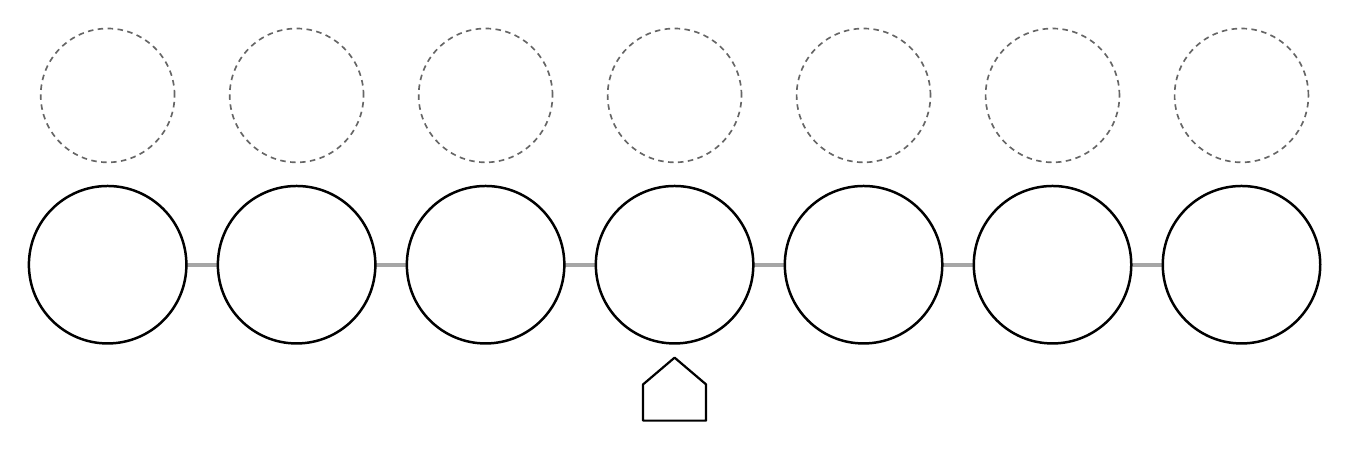
\begin{tikzpicture}[x=1mm, y=1mm]
\draw[line width=1.4pt, black!35] (-78.0,0) -- (78.0,0);
\draw[line width=0.9pt, fill=white] (-72.0,0) circle (10.0);
\draw[line width=0.6pt, black!60, dash pattern=on 2pt off 1.6pt] (-72.0,21.5) circle (8.5);
\draw[line width=0.9pt, fill=white] (-48.0,0) circle (10.0);
\draw[line width=0.6pt, black!60, dash pattern=on 2pt off 1.6pt] (-48.0,21.5) circle (8.5);
\draw[line width=0.9pt, fill=white] (-24.0,0) circle (10.0);
\draw[line width=0.6pt, black!60, dash pattern=on 2pt off 1.6pt] (-24.0,21.5) circle (8.5);
\draw[line width=0.9pt, fill=white] (0.0,0) circle (10.0);
\draw[line width=0.6pt, black!60, dash pattern=on 2pt off 1.6pt] (0.0,21.5) circle (8.5);
\draw[line width=0.9pt, fill=white] (24.0,0) circle (10.0);
\draw[line width=0.6pt, black!60, dash pattern=on 2pt off 1.6pt] (24.0,21.5) circle (8.5);
\draw[line width=0.9pt, fill=white] (48.0,0) circle (10.0);
\draw[line width=0.6pt, black!60, dash pattern=on 2pt off 1.6pt] (48.0,21.5) circle (8.5);
\draw[line width=0.9pt, fill=white] (72.0,0) circle (10.0);
\draw[line width=0.6pt, black!60, dash pattern=on 2pt off 1.6pt] (72.0,21.5) circle (8.5);
\draw[line width=0.8pt, line join=round] (0.00,-11.80) -- (4.00,-15.20) -- (4.00,-19.80) -- (-4.00,-19.80) -- (-4.00,-15.20) -- cycle;
\end{tikzpicture}}
\vspace*{2mm}
\newpage
\noindent\textbf{Problem 6:} Build each picture, starting with all lamps off, with as few moves as you can. Which one needs the most moves?

\vspace{5mm}\centerline{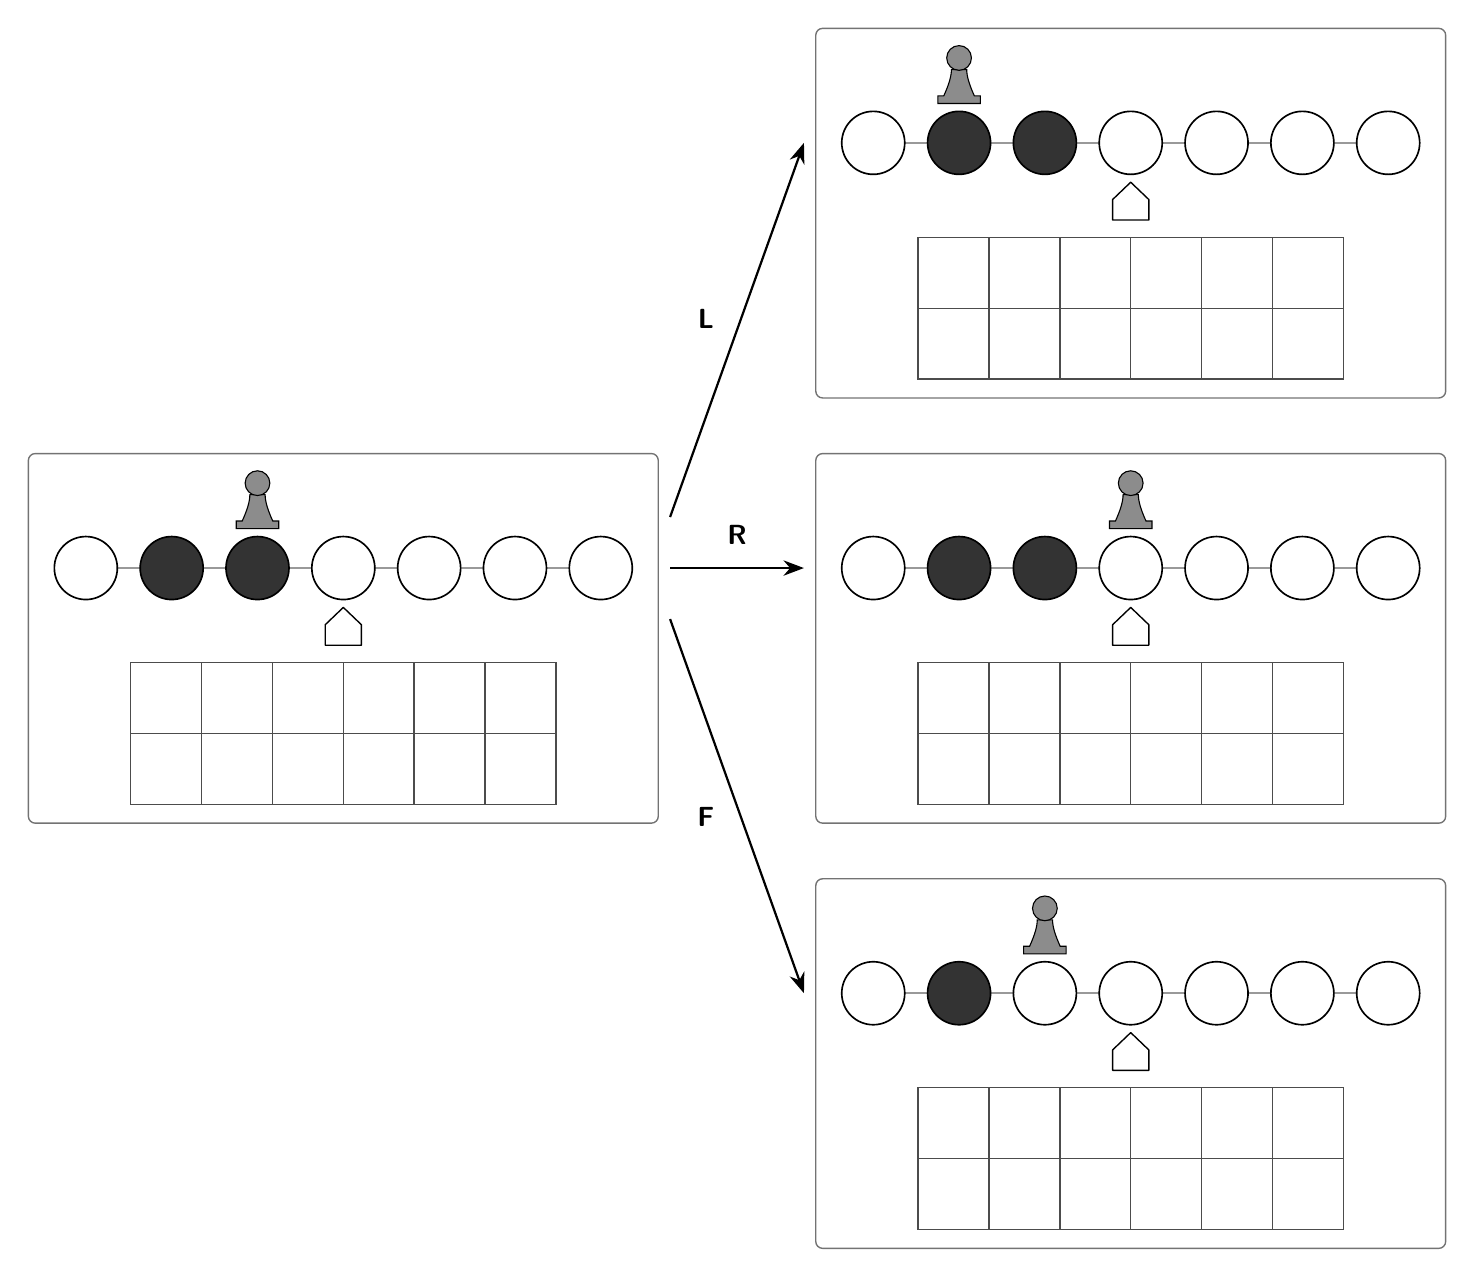
\begin{tikzpicture}[x=1mm, y=1mm]
\draw[line width=0.5pt, black!55, rounded corners=2.5] (-90.00,-32.40) rectangle (-10.00,14.54);
\draw[line width=0.9pt, black!40] (-82.70,0.00) -- (-17.30,0.00);
\draw[line width=0.6pt, fill=white] (-82.70,0.00) circle (4.0);
\draw[line width=0.6pt, fill=black!80] (-71.80,0.00) circle (4.0);
\draw[line width=0.6pt, fill=black!80] (-60.90,0.00) circle (4.0);
\draw[line width=0.6pt, fill=white] (-50.00,0.00) circle (4.0);
\draw[line width=0.6pt, fill=white] (-39.10,0.00) circle (4.0);
\draw[line width=0.6pt, fill=white] (-28.20,0.00) circle (4.0);
\draw[line width=0.6pt, fill=white] (-17.30,0.00) circle (4.0);
\draw[line width=0.4pt, fill=black!45] (-63.60,5.00) -- (-58.20,5.00) -- (-58.20,5.97) -- (-58.96,5.97) .. controls (-59.60,7.38) and (-59.93,8.46) .. (-59.93,9.32) -- (-61.87,9.32) .. controls (-61.87,8.46) and (-62.20,7.38) .. (-62.84,5.97) -- (-63.60,5.97) -- cycle;
\draw[line width=0.4pt, fill=black!45] (-60.90,10.78) circle (1.57);
\draw[line width=0.5pt, line join=round] (-50.00,-5.00) -- (-47.70,-7.20) -- (-47.70,-9.80) -- (-52.30,-9.80) -- (-52.30,-7.20) -- cycle;
\draw[line width=0.5pt, black!70] (-77.00,-21.00) rectangle (-68.00,-12.00);
\draw[line width=0.5pt, black!70] (-68.00,-21.00) rectangle (-59.00,-12.00);
\draw[line width=0.5pt, black!70] (-59.00,-21.00) rectangle (-50.00,-12.00);
\draw[line width=0.5pt, black!70] (-50.00,-21.00) rectangle (-41.00,-12.00);
\draw[line width=0.5pt, black!70] (-41.00,-21.00) rectangle (-32.00,-12.00);
\draw[line width=0.5pt, black!70] (-32.00,-21.00) rectangle (-23.00,-12.00);
\draw[line width=0.5pt, black!70] (-77.00,-30.00) rectangle (-68.00,-21.00);
\draw[line width=0.5pt, black!70] (-68.00,-30.00) rectangle (-59.00,-21.00);
\draw[line width=0.5pt, black!70] (-59.00,-30.00) rectangle (-50.00,-21.00);
\draw[line width=0.5pt, black!70] (-50.00,-30.00) rectangle (-41.00,-21.00);
\draw[line width=0.5pt, black!70] (-41.00,-30.00) rectangle (-32.00,-21.00);
\draw[line width=0.5pt, black!70] (-32.00,-30.00) rectangle (-23.00,-21.00);
\draw[line width=0.5pt, black!55, rounded corners=2.5] (10.00,21.60) rectangle (90.00,68.54);
\draw[line width=0.9pt, black!40] (17.30,54.00) -- (82.70,54.00);
\draw[line width=0.6pt, fill=white] (17.30,54.00) circle (4.0);
\draw[line width=0.6pt, fill=black!80] (28.20,54.00) circle (4.0);
\draw[line width=0.6pt, fill=black!80] (39.10,54.00) circle (4.0);
\draw[line width=0.6pt, fill=white] (50.00,54.00) circle (4.0);
\draw[line width=0.6pt, fill=white] (60.90,54.00) circle (4.0);
\draw[line width=0.6pt, fill=white] (71.80,54.00) circle (4.0);
\draw[line width=0.6pt, fill=white] (82.70,54.00) circle (4.0);
\draw[line width=0.4pt, fill=black!45] (25.50,59.00) -- (30.90,59.00) -- (30.90,59.97) -- (30.14,59.97) .. controls (29.50,61.38) and (29.17,62.46) .. (29.17,63.32) -- (27.23,63.32) .. controls (27.23,62.46) and (26.90,61.38) .. (26.26,59.97) -- (25.50,59.97) -- cycle;
\draw[line width=0.4pt, fill=black!45] (28.20,64.78) circle (1.57);
\draw[line width=0.5pt, line join=round] (50.00,49.00) -- (52.30,46.80) -- (52.30,44.20) -- (47.70,44.20) -- (47.70,46.80) -- cycle;
\draw[line width=0.5pt, black!70] (23.00,33.00) rectangle (32.00,42.00);
\draw[line width=0.5pt, black!70] (32.00,33.00) rectangle (41.00,42.00);
\draw[line width=0.5pt, black!70] (41.00,33.00) rectangle (50.00,42.00);
\draw[line width=0.5pt, black!70] (50.00,33.00) rectangle (59.00,42.00);
\draw[line width=0.5pt, black!70] (59.00,33.00) rectangle (68.00,42.00);
\draw[line width=0.5pt, black!70] (68.00,33.00) rectangle (77.00,42.00);
\draw[line width=0.5pt, black!70] (23.00,24.00) rectangle (32.00,33.00);
\draw[line width=0.5pt, black!70] (32.00,24.00) rectangle (41.00,33.00);
\draw[line width=0.5pt, black!70] (41.00,24.00) rectangle (50.00,33.00);
\draw[line width=0.5pt, black!70] (50.00,24.00) rectangle (59.00,33.00);
\draw[line width=0.5pt, black!70] (59.00,24.00) rectangle (68.00,33.00);
\draw[line width=0.5pt, black!70] (68.00,24.00) rectangle (77.00,33.00);
\draw[-{Stealth[length=2.6mm]}, line width=0.8pt] (-8.50,6.48) -- (8.50,54.00);
\node[font=\sffamily\bfseries, inner sep=0pt] at (-3.95,31.65) {L};
\draw[line width=0.5pt, black!55, rounded corners=2.5] (10.00,-32.40) rectangle (90.00,14.54);
\draw[line width=0.9pt, black!40] (17.30,0.00) -- (82.70,0.00);
\draw[line width=0.6pt, fill=white] (17.30,0.00) circle (4.0);
\draw[line width=0.6pt, fill=black!80] (28.20,0.00) circle (4.0);
\draw[line width=0.6pt, fill=black!80] (39.10,0.00) circle (4.0);
\draw[line width=0.6pt, fill=white] (50.00,0.00) circle (4.0);
\draw[line width=0.6pt, fill=white] (60.90,0.00) circle (4.0);
\draw[line width=0.6pt, fill=white] (71.80,0.00) circle (4.0);
\draw[line width=0.6pt, fill=white] (82.70,0.00) circle (4.0);
\draw[line width=0.4pt, fill=black!45] (47.30,5.00) -- (52.70,5.00) -- (52.70,5.97) -- (51.94,5.97) .. controls (51.30,7.38) and (50.97,8.46) .. (50.97,9.32) -- (49.03,9.32) .. controls (49.03,8.46) and (48.70,7.38) .. (48.06,5.97) -- (47.30,5.97) -- cycle;
\draw[line width=0.4pt, fill=black!45] (50.00,10.78) circle (1.57);
\draw[line width=0.5pt, line join=round] (50.00,-5.00) -- (52.30,-7.20) -- (52.30,-9.80) -- (47.70,-9.80) -- (47.70,-7.20) -- cycle;
\draw[line width=0.5pt, black!70] (23.00,-21.00) rectangle (32.00,-12.00);
\draw[line width=0.5pt, black!70] (32.00,-21.00) rectangle (41.00,-12.00);
\draw[line width=0.5pt, black!70] (41.00,-21.00) rectangle (50.00,-12.00);
\draw[line width=0.5pt, black!70] (50.00,-21.00) rectangle (59.00,-12.00);
\draw[line width=0.5pt, black!70] (59.00,-21.00) rectangle (68.00,-12.00);
\draw[line width=0.5pt, black!70] (68.00,-21.00) rectangle (77.00,-12.00);
\draw[line width=0.5pt, black!70] (23.00,-30.00) rectangle (32.00,-21.00);
\draw[line width=0.5pt, black!70] (32.00,-30.00) rectangle (41.00,-21.00);
\draw[line width=0.5pt, black!70] (41.00,-30.00) rectangle (50.00,-21.00);
\draw[line width=0.5pt, black!70] (50.00,-30.00) rectangle (59.00,-21.00);
\draw[line width=0.5pt, black!70] (59.00,-30.00) rectangle (68.00,-21.00);
\draw[line width=0.5pt, black!70] (68.00,-30.00) rectangle (77.00,-21.00);
\draw[-{Stealth[length=2.6mm]}, line width=0.8pt] (-8.50,0.00) -- (8.50,0.00);
\node[font=\sffamily\bfseries, inner sep=0pt] at (0.00,4.20) {R};
\draw[line width=0.5pt, black!55, rounded corners=2.5] (10.00,-86.40) rectangle (90.00,-39.46);
\draw[line width=0.9pt, black!40] (17.30,-54.00) -- (82.70,-54.00);
\draw[line width=0.6pt, fill=white] (17.30,-54.00) circle (4.0);
\draw[line width=0.6pt, fill=black!80] (28.20,-54.00) circle (4.0);
\draw[line width=0.6pt, fill=white] (39.10,-54.00) circle (4.0);
\draw[line width=0.6pt, fill=white] (50.00,-54.00) circle (4.0);
\draw[line width=0.6pt, fill=white] (60.90,-54.00) circle (4.0);
\draw[line width=0.6pt, fill=white] (71.80,-54.00) circle (4.0);
\draw[line width=0.6pt, fill=white] (82.70,-54.00) circle (4.0);
\draw[line width=0.4pt, fill=black!45] (36.40,-49.00) -- (41.80,-49.00) -- (41.80,-48.03) -- (41.04,-48.03) .. controls (40.40,-46.62) and (40.07,-45.54) .. (40.07,-44.68) -- (38.13,-44.68) .. controls (38.13,-45.54) and (37.80,-46.62) .. (37.16,-48.03) -- (36.40,-48.03) -- cycle;
\draw[line width=0.4pt, fill=black!45] (39.10,-43.22) circle (1.57);
\draw[line width=0.5pt, line join=round] (50.00,-59.00) -- (52.30,-61.20) -- (52.30,-63.80) -- (47.70,-63.80) -- (47.70,-61.20) -- cycle;
\draw[line width=0.5pt, black!70] (23.00,-75.00) rectangle (32.00,-66.00);
\draw[line width=0.5pt, black!70] (32.00,-75.00) rectangle (41.00,-66.00);
\draw[line width=0.5pt, black!70] (41.00,-75.00) rectangle (50.00,-66.00);
\draw[line width=0.5pt, black!70] (50.00,-75.00) rectangle (59.00,-66.00);
\draw[line width=0.5pt, black!70] (59.00,-75.00) rectangle (68.00,-66.00);
\draw[line width=0.5pt, black!70] (68.00,-75.00) rectangle (77.00,-66.00);
\draw[line width=0.5pt, black!70] (23.00,-84.00) rectangle (32.00,-75.00);
\draw[line width=0.5pt, black!70] (32.00,-84.00) rectangle (41.00,-75.00);
\draw[line width=0.5pt, black!70] (41.00,-84.00) rectangle (50.00,-75.00);
\draw[line width=0.5pt, black!70] (50.00,-84.00) rectangle (59.00,-75.00);
\draw[line width=0.5pt, black!70] (59.00,-84.00) rectangle (68.00,-75.00);
\draw[line width=0.5pt, black!70] (68.00,-84.00) rectangle (77.00,-75.00);
\draw[-{Stealth[length=2.6mm]}, line width=0.8pt] (-8.50,-6.48) -- (8.50,-54.00);
\node[font=\sffamily\bfseries, inner sep=0pt] at (-3.95,-31.65) {F};
\end{tikzpicture}}

\vfill
\centerline{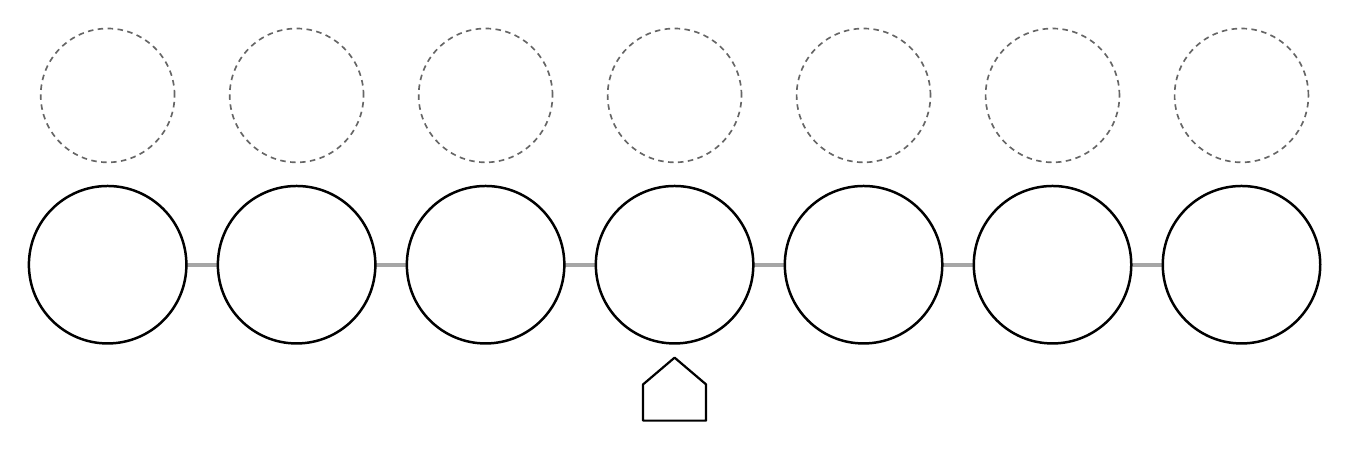
\begin{tikzpicture}[x=1mm, y=1mm]
\draw[line width=1.4pt, black!35] (-78.0,0) -- (78.0,0);
\draw[line width=0.9pt, fill=white] (-72.0,0) circle (10.0);
\draw[line width=0.6pt, black!60, dash pattern=on 2pt off 1.6pt] (-72.0,21.5) circle (8.5);
\draw[line width=0.9pt, fill=white] (-48.0,0) circle (10.0);
\draw[line width=0.6pt, black!60, dash pattern=on 2pt off 1.6pt] (-48.0,21.5) circle (8.5);
\draw[line width=0.9pt, fill=white] (-24.0,0) circle (10.0);
\draw[line width=0.6pt, black!60, dash pattern=on 2pt off 1.6pt] (-24.0,21.5) circle (8.5);
\draw[line width=0.9pt, fill=white] (0.0,0) circle (10.0);
\draw[line width=0.6pt, black!60, dash pattern=on 2pt off 1.6pt] (0.0,21.5) circle (8.5);
\draw[line width=0.9pt, fill=white] (24.0,0) circle (10.0);
\draw[line width=0.6pt, black!60, dash pattern=on 2pt off 1.6pt] (24.0,21.5) circle (8.5);
\draw[line width=0.9pt, fill=white] (48.0,0) circle (10.0);
\draw[line width=0.6pt, black!60, dash pattern=on 2pt off 1.6pt] (48.0,21.5) circle (8.5);
\draw[line width=0.9pt, fill=white] (72.0,0) circle (10.0);
\draw[line width=0.6pt, black!60, dash pattern=on 2pt off 1.6pt] (72.0,21.5) circle (8.5);
\draw[line width=0.8pt, line join=round] (0.00,-11.80) -- (4.00,-15.20) -- (4.00,-19.80) -- (-4.00,-19.80) -- (-4.00,-15.20) -- cycle;
\end{tikzpicture}}
\vspace*{2mm}
\newpage
\noindent\textbf{Problem 7:} Build each picture, starting with all lamps off, with as few moves as you can. Which one needs the most moves?

\vspace{5mm}\centerline{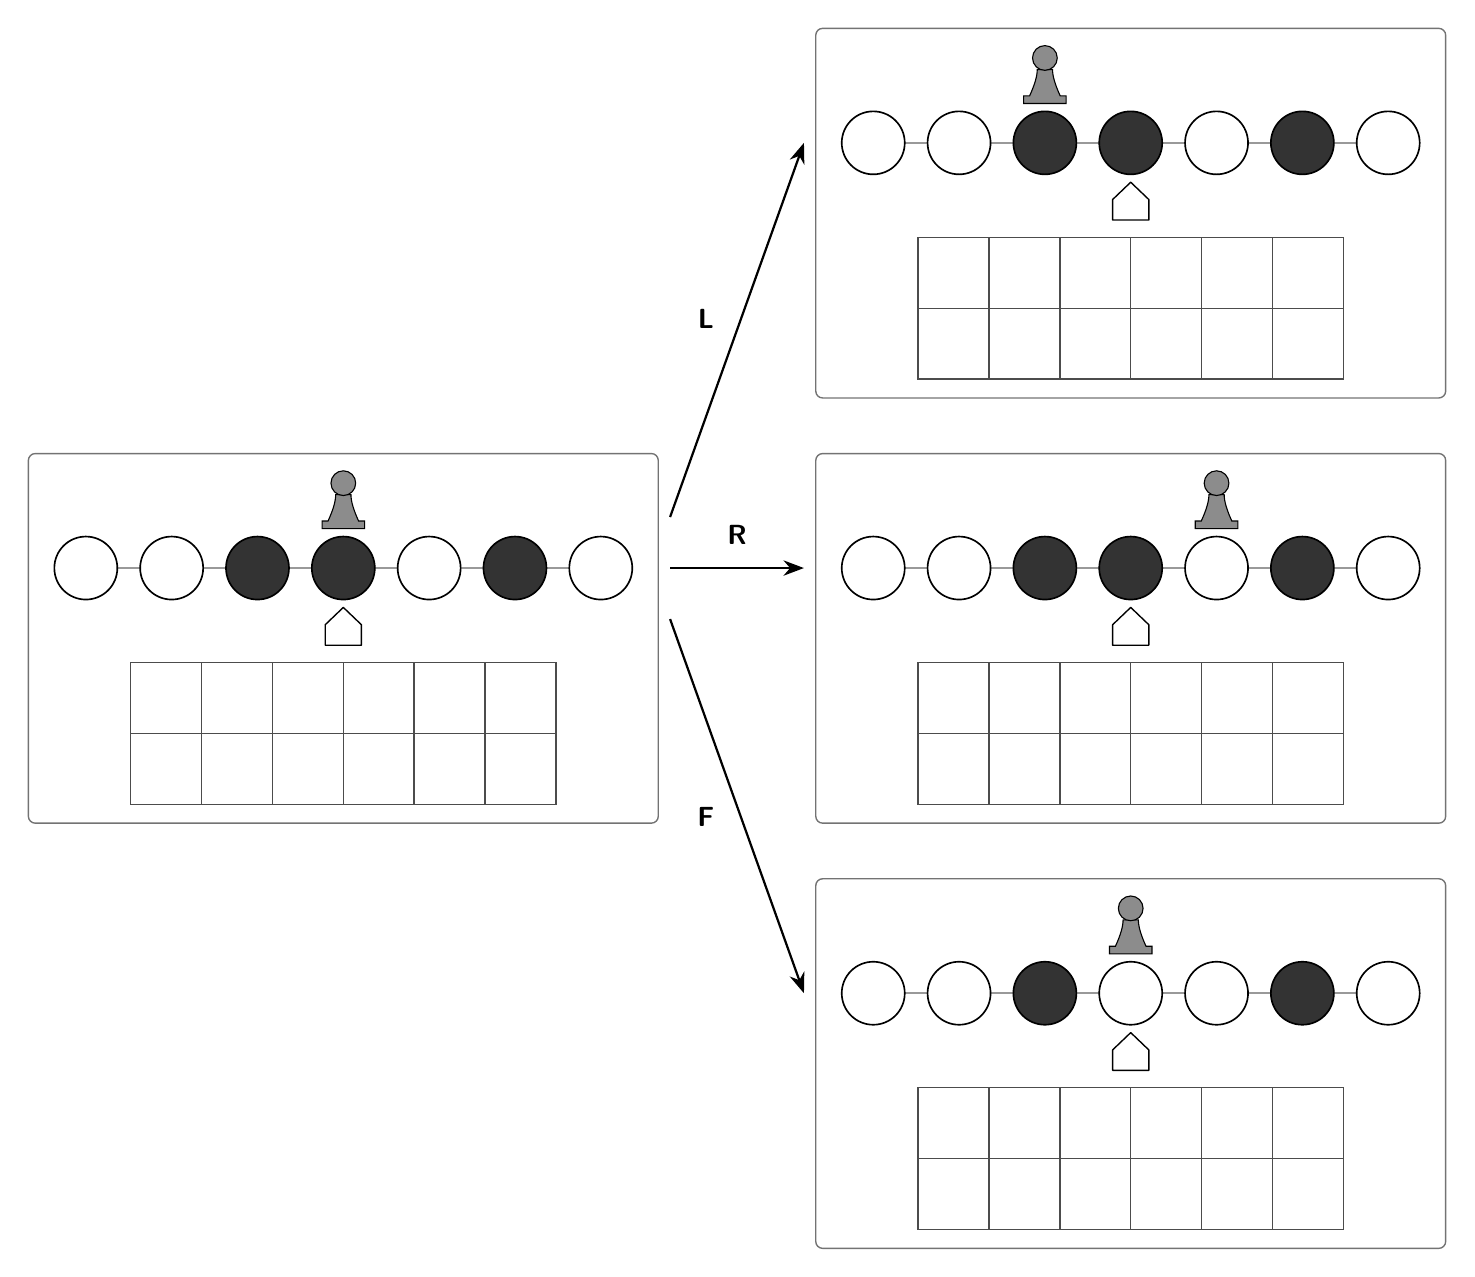
\begin{tikzpicture}[x=1mm, y=1mm]
\draw[line width=0.5pt, black!55, rounded corners=2.5] (-90.00,-32.40) rectangle (-10.00,14.54);
\draw[line width=0.9pt, black!40] (-82.70,0.00) -- (-17.30,0.00);
\draw[line width=0.6pt, fill=white] (-82.70,0.00) circle (4.0);
\draw[line width=0.6pt, fill=white] (-71.80,0.00) circle (4.0);
\draw[line width=0.6pt, fill=black!80] (-60.90,0.00) circle (4.0);
\draw[line width=0.6pt, fill=black!80] (-50.00,0.00) circle (4.0);
\draw[line width=0.6pt, fill=white] (-39.10,0.00) circle (4.0);
\draw[line width=0.6pt, fill=black!80] (-28.20,0.00) circle (4.0);
\draw[line width=0.6pt, fill=white] (-17.30,0.00) circle (4.0);
\draw[line width=0.4pt, fill=black!45] (-52.70,5.00) -- (-47.30,5.00) -- (-47.30,5.97) -- (-48.06,5.97) .. controls (-48.70,7.38) and (-49.03,8.46) .. (-49.03,9.32) -- (-50.97,9.32) .. controls (-50.97,8.46) and (-51.30,7.38) .. (-51.94,5.97) -- (-52.70,5.97) -- cycle;
\draw[line width=0.4pt, fill=black!45] (-50.00,10.78) circle (1.57);
\draw[line width=0.5pt, line join=round] (-50.00,-5.00) -- (-47.70,-7.20) -- (-47.70,-9.80) -- (-52.30,-9.80) -- (-52.30,-7.20) -- cycle;
\draw[line width=0.5pt, black!70] (-77.00,-21.00) rectangle (-68.00,-12.00);
\draw[line width=0.5pt, black!70] (-68.00,-21.00) rectangle (-59.00,-12.00);
\draw[line width=0.5pt, black!70] (-59.00,-21.00) rectangle (-50.00,-12.00);
\draw[line width=0.5pt, black!70] (-50.00,-21.00) rectangle (-41.00,-12.00);
\draw[line width=0.5pt, black!70] (-41.00,-21.00) rectangle (-32.00,-12.00);
\draw[line width=0.5pt, black!70] (-32.00,-21.00) rectangle (-23.00,-12.00);
\draw[line width=0.5pt, black!70] (-77.00,-30.00) rectangle (-68.00,-21.00);
\draw[line width=0.5pt, black!70] (-68.00,-30.00) rectangle (-59.00,-21.00);
\draw[line width=0.5pt, black!70] (-59.00,-30.00) rectangle (-50.00,-21.00);
\draw[line width=0.5pt, black!70] (-50.00,-30.00) rectangle (-41.00,-21.00);
\draw[line width=0.5pt, black!70] (-41.00,-30.00) rectangle (-32.00,-21.00);
\draw[line width=0.5pt, black!70] (-32.00,-30.00) rectangle (-23.00,-21.00);
\draw[line width=0.5pt, black!55, rounded corners=2.5] (10.00,21.60) rectangle (90.00,68.54);
\draw[line width=0.9pt, black!40] (17.30,54.00) -- (82.70,54.00);
\draw[line width=0.6pt, fill=white] (17.30,54.00) circle (4.0);
\draw[line width=0.6pt, fill=white] (28.20,54.00) circle (4.0);
\draw[line width=0.6pt, fill=black!80] (39.10,54.00) circle (4.0);
\draw[line width=0.6pt, fill=black!80] (50.00,54.00) circle (4.0);
\draw[line width=0.6pt, fill=white] (60.90,54.00) circle (4.0);
\draw[line width=0.6pt, fill=black!80] (71.80,54.00) circle (4.0);
\draw[line width=0.6pt, fill=white] (82.70,54.00) circle (4.0);
\draw[line width=0.4pt, fill=black!45] (36.40,59.00) -- (41.80,59.00) -- (41.80,59.97) -- (41.04,59.97) .. controls (40.40,61.38) and (40.07,62.46) .. (40.07,63.32) -- (38.13,63.32) .. controls (38.13,62.46) and (37.80,61.38) .. (37.16,59.97) -- (36.40,59.97) -- cycle;
\draw[line width=0.4pt, fill=black!45] (39.10,64.78) circle (1.57);
\draw[line width=0.5pt, line join=round] (50.00,49.00) -- (52.30,46.80) -- (52.30,44.20) -- (47.70,44.20) -- (47.70,46.80) -- cycle;
\draw[line width=0.5pt, black!70] (23.00,33.00) rectangle (32.00,42.00);
\draw[line width=0.5pt, black!70] (32.00,33.00) rectangle (41.00,42.00);
\draw[line width=0.5pt, black!70] (41.00,33.00) rectangle (50.00,42.00);
\draw[line width=0.5pt, black!70] (50.00,33.00) rectangle (59.00,42.00);
\draw[line width=0.5pt, black!70] (59.00,33.00) rectangle (68.00,42.00);
\draw[line width=0.5pt, black!70] (68.00,33.00) rectangle (77.00,42.00);
\draw[line width=0.5pt, black!70] (23.00,24.00) rectangle (32.00,33.00);
\draw[line width=0.5pt, black!70] (32.00,24.00) rectangle (41.00,33.00);
\draw[line width=0.5pt, black!70] (41.00,24.00) rectangle (50.00,33.00);
\draw[line width=0.5pt, black!70] (50.00,24.00) rectangle (59.00,33.00);
\draw[line width=0.5pt, black!70] (59.00,24.00) rectangle (68.00,33.00);
\draw[line width=0.5pt, black!70] (68.00,24.00) rectangle (77.00,33.00);
\draw[-{Stealth[length=2.6mm]}, line width=0.8pt] (-8.50,6.48) -- (8.50,54.00);
\node[font=\sffamily\bfseries, inner sep=0pt] at (-3.95,31.65) {L};
\draw[line width=0.5pt, black!55, rounded corners=2.5] (10.00,-32.40) rectangle (90.00,14.54);
\draw[line width=0.9pt, black!40] (17.30,0.00) -- (82.70,0.00);
\draw[line width=0.6pt, fill=white] (17.30,0.00) circle (4.0);
\draw[line width=0.6pt, fill=white] (28.20,0.00) circle (4.0);
\draw[line width=0.6pt, fill=black!80] (39.10,0.00) circle (4.0);
\draw[line width=0.6pt, fill=black!80] (50.00,0.00) circle (4.0);
\draw[line width=0.6pt, fill=white] (60.90,0.00) circle (4.0);
\draw[line width=0.6pt, fill=black!80] (71.80,0.00) circle (4.0);
\draw[line width=0.6pt, fill=white] (82.70,0.00) circle (4.0);
\draw[line width=0.4pt, fill=black!45] (58.20,5.00) -- (63.60,5.00) -- (63.60,5.97) -- (62.84,5.97) .. controls (62.20,7.38) and (61.87,8.46) .. (61.87,9.32) -- (59.93,9.32) .. controls (59.93,8.46) and (59.60,7.38) .. (58.96,5.97) -- (58.20,5.97) -- cycle;
\draw[line width=0.4pt, fill=black!45] (60.90,10.78) circle (1.57);
\draw[line width=0.5pt, line join=round] (50.00,-5.00) -- (52.30,-7.20) -- (52.30,-9.80) -- (47.70,-9.80) -- (47.70,-7.20) -- cycle;
\draw[line width=0.5pt, black!70] (23.00,-21.00) rectangle (32.00,-12.00);
\draw[line width=0.5pt, black!70] (32.00,-21.00) rectangle (41.00,-12.00);
\draw[line width=0.5pt, black!70] (41.00,-21.00) rectangle (50.00,-12.00);
\draw[line width=0.5pt, black!70] (50.00,-21.00) rectangle (59.00,-12.00);
\draw[line width=0.5pt, black!70] (59.00,-21.00) rectangle (68.00,-12.00);
\draw[line width=0.5pt, black!70] (68.00,-21.00) rectangle (77.00,-12.00);
\draw[line width=0.5pt, black!70] (23.00,-30.00) rectangle (32.00,-21.00);
\draw[line width=0.5pt, black!70] (32.00,-30.00) rectangle (41.00,-21.00);
\draw[line width=0.5pt, black!70] (41.00,-30.00) rectangle (50.00,-21.00);
\draw[line width=0.5pt, black!70] (50.00,-30.00) rectangle (59.00,-21.00);
\draw[line width=0.5pt, black!70] (59.00,-30.00) rectangle (68.00,-21.00);
\draw[line width=0.5pt, black!70] (68.00,-30.00) rectangle (77.00,-21.00);
\draw[-{Stealth[length=2.6mm]}, line width=0.8pt] (-8.50,0.00) -- (8.50,0.00);
\node[font=\sffamily\bfseries, inner sep=0pt] at (0.00,4.20) {R};
\draw[line width=0.5pt, black!55, rounded corners=2.5] (10.00,-86.40) rectangle (90.00,-39.46);
\draw[line width=0.9pt, black!40] (17.30,-54.00) -- (82.70,-54.00);
\draw[line width=0.6pt, fill=white] (17.30,-54.00) circle (4.0);
\draw[line width=0.6pt, fill=white] (28.20,-54.00) circle (4.0);
\draw[line width=0.6pt, fill=black!80] (39.10,-54.00) circle (4.0);
\draw[line width=0.6pt, fill=white] (50.00,-54.00) circle (4.0);
\draw[line width=0.6pt, fill=white] (60.90,-54.00) circle (4.0);
\draw[line width=0.6pt, fill=black!80] (71.80,-54.00) circle (4.0);
\draw[line width=0.6pt, fill=white] (82.70,-54.00) circle (4.0);
\draw[line width=0.4pt, fill=black!45] (47.30,-49.00) -- (52.70,-49.00) -- (52.70,-48.03) -- (51.94,-48.03) .. controls (51.30,-46.62) and (50.97,-45.54) .. (50.97,-44.68) -- (49.03,-44.68) .. controls (49.03,-45.54) and (48.70,-46.62) .. (48.06,-48.03) -- (47.30,-48.03) -- cycle;
\draw[line width=0.4pt, fill=black!45] (50.00,-43.22) circle (1.57);
\draw[line width=0.5pt, line join=round] (50.00,-59.00) -- (52.30,-61.20) -- (52.30,-63.80) -- (47.70,-63.80) -- (47.70,-61.20) -- cycle;
\draw[line width=0.5pt, black!70] (23.00,-75.00) rectangle (32.00,-66.00);
\draw[line width=0.5pt, black!70] (32.00,-75.00) rectangle (41.00,-66.00);
\draw[line width=0.5pt, black!70] (41.00,-75.00) rectangle (50.00,-66.00);
\draw[line width=0.5pt, black!70] (50.00,-75.00) rectangle (59.00,-66.00);
\draw[line width=0.5pt, black!70] (59.00,-75.00) rectangle (68.00,-66.00);
\draw[line width=0.5pt, black!70] (68.00,-75.00) rectangle (77.00,-66.00);
\draw[line width=0.5pt, black!70] (23.00,-84.00) rectangle (32.00,-75.00);
\draw[line width=0.5pt, black!70] (32.00,-84.00) rectangle (41.00,-75.00);
\draw[line width=0.5pt, black!70] (41.00,-84.00) rectangle (50.00,-75.00);
\draw[line width=0.5pt, black!70] (50.00,-84.00) rectangle (59.00,-75.00);
\draw[line width=0.5pt, black!70] (59.00,-84.00) rectangle (68.00,-75.00);
\draw[line width=0.5pt, black!70] (68.00,-84.00) rectangle (77.00,-75.00);
\draw[-{Stealth[length=2.6mm]}, line width=0.8pt] (-8.50,-6.48) -- (8.50,-54.00);
\node[font=\sffamily\bfseries, inner sep=0pt] at (-3.95,-31.65) {F};
\end{tikzpicture}}

\vfill
\centerline{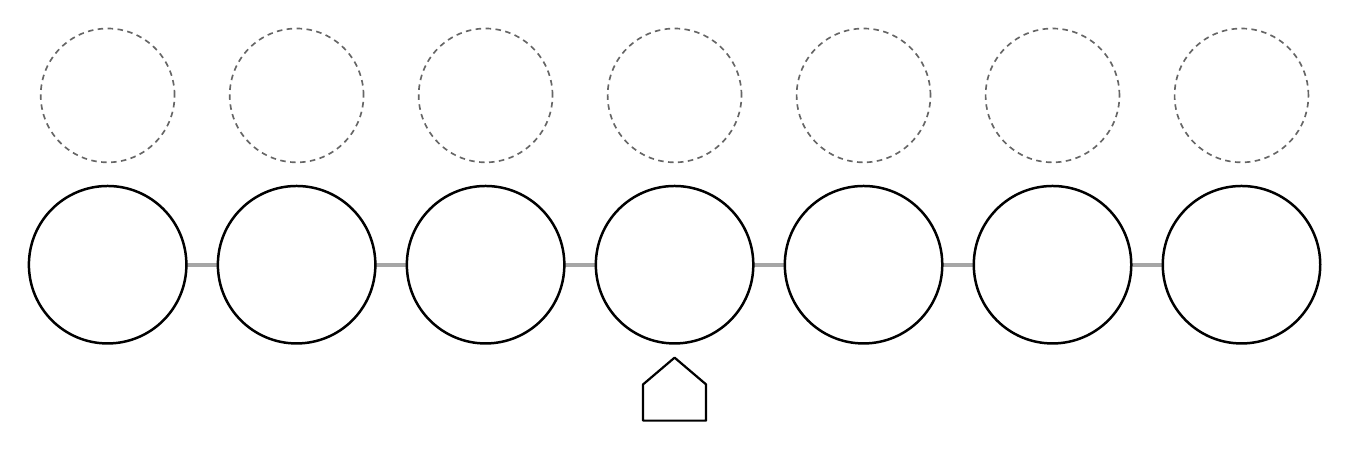
\begin{tikzpicture}[x=1mm, y=1mm]
\draw[line width=1.4pt, black!35] (-78.0,0) -- (78.0,0);
\draw[line width=0.9pt, fill=white] (-72.0,0) circle (10.0);
\draw[line width=0.6pt, black!60, dash pattern=on 2pt off 1.6pt] (-72.0,21.5) circle (8.5);
\draw[line width=0.9pt, fill=white] (-48.0,0) circle (10.0);
\draw[line width=0.6pt, black!60, dash pattern=on 2pt off 1.6pt] (-48.0,21.5) circle (8.5);
\draw[line width=0.9pt, fill=white] (-24.0,0) circle (10.0);
\draw[line width=0.6pt, black!60, dash pattern=on 2pt off 1.6pt] (-24.0,21.5) circle (8.5);
\draw[line width=0.9pt, fill=white] (0.0,0) circle (10.0);
\draw[line width=0.6pt, black!60, dash pattern=on 2pt off 1.6pt] (0.0,21.5) circle (8.5);
\draw[line width=0.9pt, fill=white] (24.0,0) circle (10.0);
\draw[line width=0.6pt, black!60, dash pattern=on 2pt off 1.6pt] (24.0,21.5) circle (8.5);
\draw[line width=0.9pt, fill=white] (48.0,0) circle (10.0);
\draw[line width=0.6pt, black!60, dash pattern=on 2pt off 1.6pt] (48.0,21.5) circle (8.5);
\draw[line width=0.9pt, fill=white] (72.0,0) circle (10.0);
\draw[line width=0.6pt, black!60, dash pattern=on 2pt off 1.6pt] (72.0,21.5) circle (8.5);
\draw[line width=0.8pt, line join=round] (0.00,-11.80) -- (4.00,-15.20) -- (4.00,-19.80) -- (-4.00,-19.80) -- (-4.00,-15.20) -- cycle;
\end{tikzpicture}}
\vspace*{2mm}
\newpage
\noindent\textbf{Problem 8:} For each tower, try to build the picture in its row with exactly that many moves. Circle every tower that works.

\vspace{6mm}\centerline{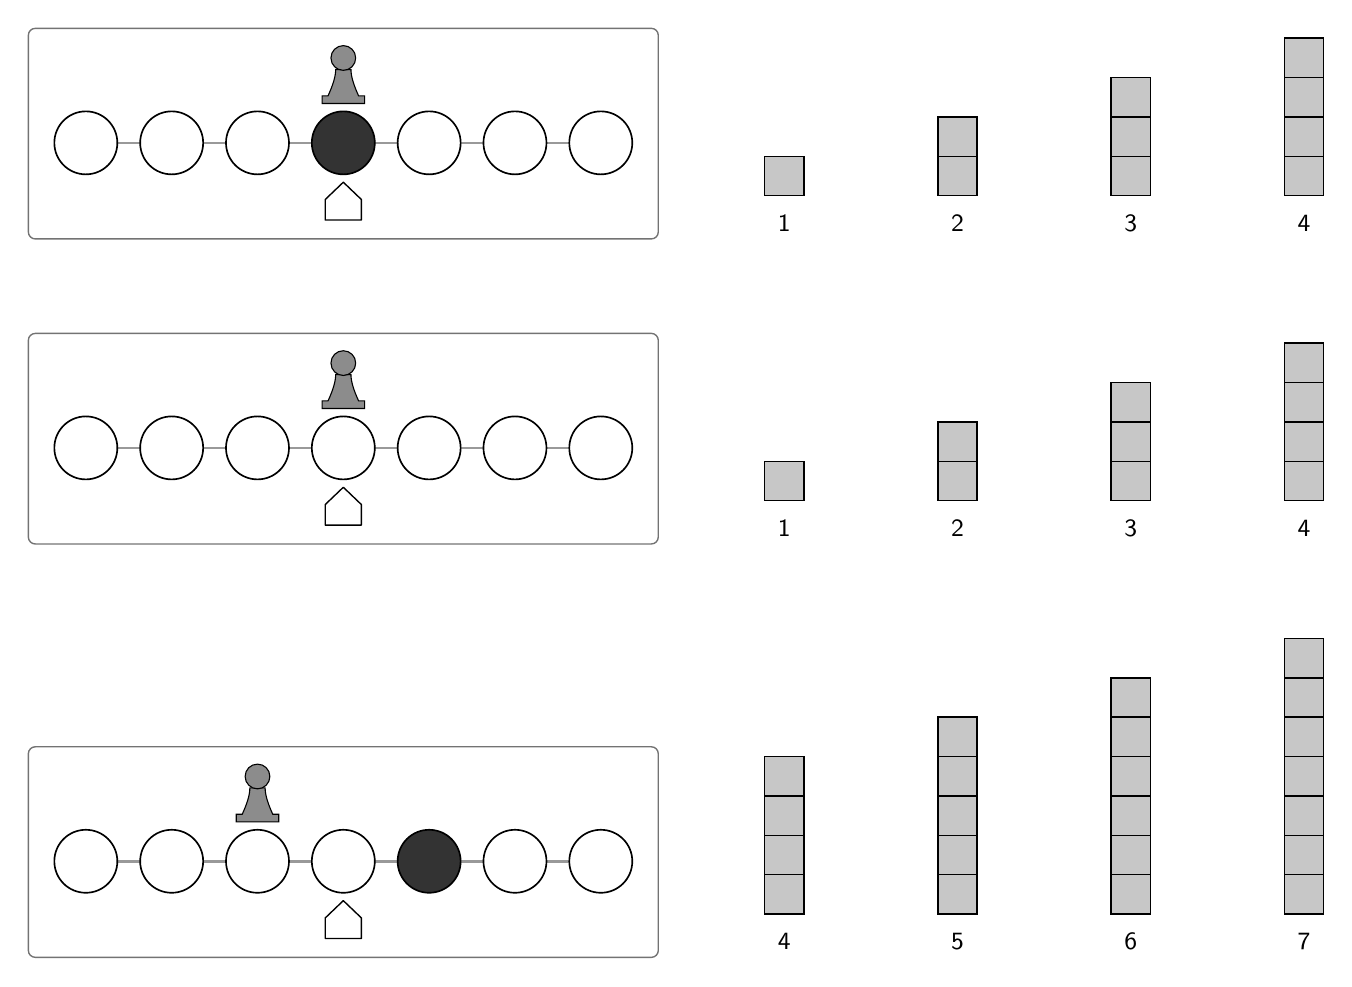
\begin{tikzpicture}[x=1mm, y=1mm]
\draw[line width=0.5pt, black!55, rounded corners=2.5] (-90.00,-12.20) rectangle (-10.00,14.54);
\draw[line width=0.9pt, black!40] (-82.70,0.00) -- (-17.30,0.00);
\draw[line width=0.6pt, fill=white] (-82.70,0.00) circle (4.0);
\draw[line width=0.6pt, fill=white] (-71.80,0.00) circle (4.0);
\draw[line width=0.6pt, fill=white] (-60.90,0.00) circle (4.0);
\draw[line width=0.6pt, fill=black!80] (-50.00,0.00) circle (4.0);
\draw[line width=0.6pt, fill=white] (-39.10,0.00) circle (4.0);
\draw[line width=0.6pt, fill=white] (-28.20,0.00) circle (4.0);
\draw[line width=0.6pt, fill=white] (-17.30,0.00) circle (4.0);
\draw[line width=0.4pt, fill=black!45] (-52.70,5.00) -- (-47.30,5.00) -- (-47.30,5.97) -- (-48.06,5.97) .. controls (-48.70,7.38) and (-49.03,8.46) .. (-49.03,9.32) -- (-50.97,9.32) .. controls (-50.97,8.46) and (-51.30,7.38) .. (-51.94,5.97) -- (-52.70,5.97) -- cycle;
\draw[line width=0.4pt, fill=black!45] (-50.00,10.78) circle (1.57);
\draw[line width=0.5pt, line join=round] (-50.00,-5.00) -- (-47.70,-7.20) -- (-47.70,-9.80) -- (-52.30,-9.80) -- (-52.30,-7.20) -- cycle;
\draw[line width=0.5pt, fill=black!22] (3.50,-6.70) rectangle (8.50,-1.70);
\node[font=\sffamily\small, anchor=north] at (6.00,-7.90) {1};
\draw[line width=0.5pt, fill=black!22] (25.50,-6.70) rectangle (30.50,-1.70);
\draw[line width=0.5pt, fill=black!22] (25.50,-1.70) rectangle (30.50,3.30);
\node[font=\sffamily\small, anchor=north] at (28.00,-7.90) {2};
\draw[line width=0.5pt, fill=black!22] (47.50,-6.70) rectangle (52.50,-1.70);
\draw[line width=0.5pt, fill=black!22] (47.50,-1.70) rectangle (52.50,3.30);
\draw[line width=0.5pt, fill=black!22] (47.50,3.30) rectangle (52.50,8.30);
\node[font=\sffamily\small, anchor=north] at (50.00,-7.90) {3};
\draw[line width=0.5pt, fill=black!22] (69.50,-6.70) rectangle (74.50,-1.70);
\draw[line width=0.5pt, fill=black!22] (69.50,-1.70) rectangle (74.50,3.30);
\draw[line width=0.5pt, fill=black!22] (69.50,3.30) rectangle (74.50,8.30);
\draw[line width=0.5pt, fill=black!22] (69.50,8.30) rectangle (74.50,13.30);
\node[font=\sffamily\small, anchor=north] at (72.00,-7.90) {4};
\draw[line width=0.5pt, black!55, rounded corners=2.5] (-90.00,-50.94) rectangle (-10.00,-24.20);
\draw[line width=0.9pt, black!40] (-82.70,-38.74) -- (-17.30,-38.74);
\draw[line width=0.6pt, fill=white] (-82.70,-38.74) circle (4.0);
\draw[line width=0.6pt, fill=white] (-71.80,-38.74) circle (4.0);
\draw[line width=0.6pt, fill=white] (-60.90,-38.74) circle (4.0);
\draw[line width=0.6pt, fill=white] (-50.00,-38.74) circle (4.0);
\draw[line width=0.6pt, fill=white] (-39.10,-38.74) circle (4.0);
\draw[line width=0.6pt, fill=white] (-28.20,-38.74) circle (4.0);
\draw[line width=0.6pt, fill=white] (-17.30,-38.74) circle (4.0);
\draw[line width=0.4pt, fill=black!45] (-52.70,-33.74) -- (-47.30,-33.74) -- (-47.30,-32.77) -- (-48.06,-32.77) .. controls (-48.70,-31.37) and (-49.03,-30.29) .. (-49.03,-29.42) -- (-50.97,-29.42) .. controls (-50.97,-30.29) and (-51.30,-31.37) .. (-51.94,-32.77) -- (-52.70,-32.77) -- cycle;
\draw[line width=0.4pt, fill=black!45] (-50.00,-27.97) circle (1.57);
\draw[line width=0.5pt, line join=round] (-50.00,-43.74) -- (-47.70,-45.94) -- (-47.70,-48.54) -- (-52.30,-48.54) -- (-52.30,-45.94) -- cycle;
\draw[line width=0.5pt, fill=black!22] (3.50,-45.44) rectangle (8.50,-40.44);
\node[font=\sffamily\small, anchor=north] at (6.00,-46.64) {1};
\draw[line width=0.5pt, fill=black!22] (25.50,-45.44) rectangle (30.50,-40.44);
\draw[line width=0.5pt, fill=black!22] (25.50,-40.44) rectangle (30.50,-35.44);
\node[font=\sffamily\small, anchor=north] at (28.00,-46.64) {2};
\draw[line width=0.5pt, fill=black!22] (47.50,-45.44) rectangle (52.50,-40.44);
\draw[line width=0.5pt, fill=black!22] (47.50,-40.44) rectangle (52.50,-35.44);
\draw[line width=0.5pt, fill=black!22] (47.50,-35.44) rectangle (52.50,-30.44);
\node[font=\sffamily\small, anchor=north] at (50.00,-46.64) {3};
\draw[line width=0.5pt, fill=black!22] (69.50,-45.44) rectangle (74.50,-40.44);
\draw[line width=0.5pt, fill=black!22] (69.50,-40.44) rectangle (74.50,-35.44);
\draw[line width=0.5pt, fill=black!22] (69.50,-35.44) rectangle (74.50,-30.44);
\draw[line width=0.5pt, fill=black!22] (69.50,-30.44) rectangle (74.50,-25.44);
\node[font=\sffamily\small, anchor=north] at (72.00,-46.64) {4};
\draw[line width=0.5pt, black!55, rounded corners=2.5] (-90.00,-103.44) rectangle (-10.00,-76.70);
\draw[line width=0.9pt, black!40] (-82.70,-91.24) -- (-17.30,-91.24);
\draw[line width=0.6pt, fill=white] (-82.70,-91.24) circle (4.0);
\draw[line width=0.6pt, fill=white] (-71.80,-91.24) circle (4.0);
\draw[line width=0.6pt, fill=white] (-60.90,-91.24) circle (4.0);
\draw[line width=0.6pt, fill=white] (-50.00,-91.24) circle (4.0);
\draw[line width=0.6pt, fill=black!80] (-39.10,-91.24) circle (4.0);
\draw[line width=0.6pt, fill=white] (-28.20,-91.24) circle (4.0);
\draw[line width=0.6pt, fill=white] (-17.30,-91.24) circle (4.0);
\draw[line width=0.4pt, fill=black!45] (-63.60,-86.24) -- (-58.20,-86.24) -- (-58.20,-85.27) -- (-58.96,-85.27) .. controls (-59.60,-83.87) and (-59.93,-82.79) .. (-59.93,-81.92) -- (-61.87,-81.92) .. controls (-61.87,-82.79) and (-62.20,-83.87) .. (-62.84,-85.27) -- (-63.60,-85.27) -- cycle;
\draw[line width=0.4pt, fill=black!45] (-60.90,-80.47) circle (1.57);
\draw[line width=0.5pt, line join=round] (-50.00,-96.24) -- (-47.70,-98.44) -- (-47.70,-101.04) -- (-52.30,-101.04) -- (-52.30,-98.44) -- cycle;
\draw[line width=0.5pt, fill=black!22] (3.50,-97.94) rectangle (8.50,-92.94);
\draw[line width=0.5pt, fill=black!22] (3.50,-92.94) rectangle (8.50,-87.94);
\draw[line width=0.5pt, fill=black!22] (3.50,-87.94) rectangle (8.50,-82.94);
\draw[line width=0.5pt, fill=black!22] (3.50,-82.94) rectangle (8.50,-77.94);
\node[font=\sffamily\small, anchor=north] at (6.00,-99.14) {4};
\draw[line width=0.5pt, fill=black!22] (25.50,-97.94) rectangle (30.50,-92.94);
\draw[line width=0.5pt, fill=black!22] (25.50,-92.94) rectangle (30.50,-87.94);
\draw[line width=0.5pt, fill=black!22] (25.50,-87.94) rectangle (30.50,-82.94);
\draw[line width=0.5pt, fill=black!22] (25.50,-82.94) rectangle (30.50,-77.94);
\draw[line width=0.5pt, fill=black!22] (25.50,-77.94) rectangle (30.50,-72.94);
\node[font=\sffamily\small, anchor=north] at (28.00,-99.14) {5};
\draw[line width=0.5pt, fill=black!22] (47.50,-97.94) rectangle (52.50,-92.94);
\draw[line width=0.5pt, fill=black!22] (47.50,-92.94) rectangle (52.50,-87.94);
\draw[line width=0.5pt, fill=black!22] (47.50,-87.94) rectangle (52.50,-82.94);
\draw[line width=0.5pt, fill=black!22] (47.50,-82.94) rectangle (52.50,-77.94);
\draw[line width=0.5pt, fill=black!22] (47.50,-77.94) rectangle (52.50,-72.94);
\draw[line width=0.5pt, fill=black!22] (47.50,-72.94) rectangle (52.50,-67.94);
\node[font=\sffamily\small, anchor=north] at (50.00,-99.14) {6};
\draw[line width=0.5pt, fill=black!22] (69.50,-97.94) rectangle (74.50,-92.94);
\draw[line width=0.5pt, fill=black!22] (69.50,-92.94) rectangle (74.50,-87.94);
\draw[line width=0.5pt, fill=black!22] (69.50,-87.94) rectangle (74.50,-82.94);
\draw[line width=0.5pt, fill=black!22] (69.50,-82.94) rectangle (74.50,-77.94);
\draw[line width=0.5pt, fill=black!22] (69.50,-77.94) rectangle (74.50,-72.94);
\draw[line width=0.5pt, fill=black!22] (69.50,-72.94) rectangle (74.50,-67.94);
\draw[line width=0.5pt, fill=black!22] (69.50,-67.94) rectangle (74.50,-62.94);
\node[font=\sffamily\small, anchor=north] at (72.00,-99.14) {7};
\end{tikzpicture}}

\vfill
\centerline{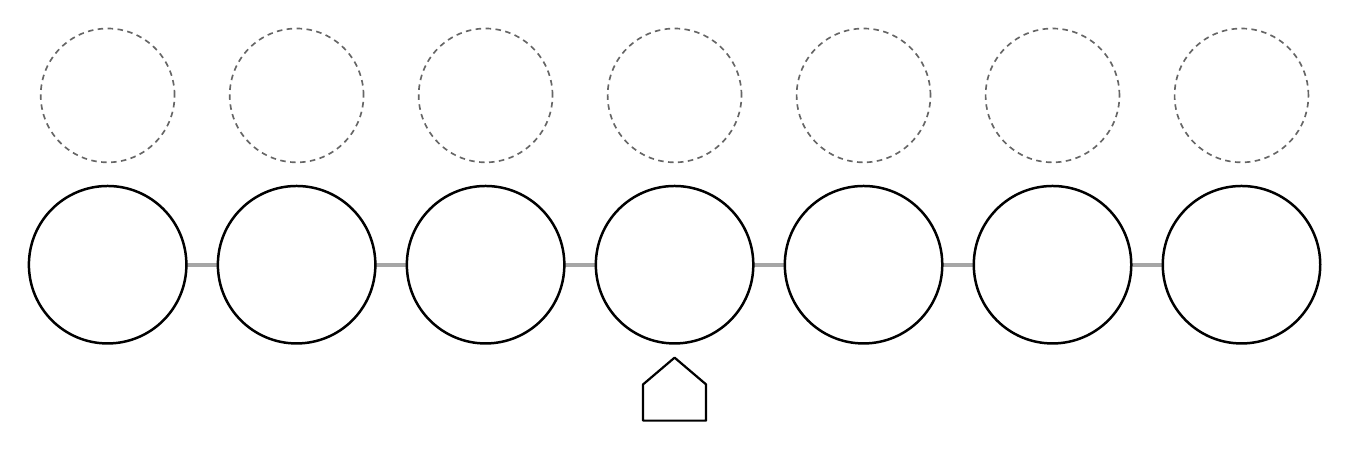
\begin{tikzpicture}[x=1mm, y=1mm]
\draw[line width=1.4pt, black!35] (-78.0,0) -- (78.0,0);
\draw[line width=0.9pt, fill=white] (-72.0,0) circle (10.0);
\draw[line width=0.6pt, black!60, dash pattern=on 2pt off 1.6pt] (-72.0,21.5) circle (8.5);
\draw[line width=0.9pt, fill=white] (-48.0,0) circle (10.0);
\draw[line width=0.6pt, black!60, dash pattern=on 2pt off 1.6pt] (-48.0,21.5) circle (8.5);
\draw[line width=0.9pt, fill=white] (-24.0,0) circle (10.0);
\draw[line width=0.6pt, black!60, dash pattern=on 2pt off 1.6pt] (-24.0,21.5) circle (8.5);
\draw[line width=0.9pt, fill=white] (0.0,0) circle (10.0);
\draw[line width=0.6pt, black!60, dash pattern=on 2pt off 1.6pt] (0.0,21.5) circle (8.5);
\draw[line width=0.9pt, fill=white] (24.0,0) circle (10.0);
\draw[line width=0.6pt, black!60, dash pattern=on 2pt off 1.6pt] (24.0,21.5) circle (8.5);
\draw[line width=0.9pt, fill=white] (48.0,0) circle (10.0);
\draw[line width=0.6pt, black!60, dash pattern=on 2pt off 1.6pt] (48.0,21.5) circle (8.5);
\draw[line width=0.9pt, fill=white] (72.0,0) circle (10.0);
\draw[line width=0.6pt, black!60, dash pattern=on 2pt off 1.6pt] (72.0,21.5) circle (8.5);
\draw[line width=0.8pt, line join=round] (0.00,-11.80) -- (4.00,-15.20) -- (4.00,-19.80) -- (-4.00,-19.80) -- (-4.00,-15.20) -- cycle;
\end{tikzpicture}}
\vspace*{2mm}
\end{document}
